\chapter{اندروید}
\section{ساختار راهنمای برنامه‌ی اندروید}
این راهنما به شما کمک می‌کند تا به راحتی از برنامه ما استفاده کنید. هدف ما این است که تجربه‌ای روان و دلپذیر را برای شما فراهم کنیم. این برنامه به شما امکان می‌دهد تا به سرعت و سادگی کارهای مورد نظر خود را انجام دهید.  
برنامه شامل بخش‌های مختلفی است که هر یک برای نیاز خاصی طراحی شده‌اند. صفحه \lr{Login} به شما امکان ورود سریع و امن به حساب کاربری را می‌دهد. بخش \lr{Sign Up} شامل فرم ثبت‌نام و مرحله تأیید ایمیل است تا امنیت و صحت اطلاعات تضمین شود. در صورت فراموشی رمز عبور، بخش \lr{Reset Password} با سه مرحله‌ی احراز هویت، تأیید کد و تغییر رمز عبور، فرآیند بازیابی را ساده و امن می‌کند. صفحه‌ی \lr{Home} محل اجرای تست‌ها و اندازه گیری‌ها و مرکز اصلی دسترسی به امکانات برنامه است و قابلیت خروج از حساب نیز در آن گنجانده شده است. بخش \lr{Settings} به کاربران اجازه می‌دهد تنظیمات دلخواه خود را اعمال کنند و قسمت \lr{Permission} برای مدیریت مجوزهای مورد نیاز برنامه طراحی شده است. این ساختار به گونه‌ای ایجاد شده که کاربران بتوانند بدون پیچیدگی و با حداقل زمان، به تمام امکانات برنامه دسترسی داشته باشند.

\section{شروع به کار}
\begin{itemize}
	\item  مجوزهای برنامه: 
	برنامه‌ی اندروید Polaris برای اجرای صحیح وظایف خود به مجموعه‌ای از مجوزها نیاز دارد. این مجوزها و کاربرد آن‌ها به شرح زیر است:
	\begin{itemize}
		\item \textbf{دسترسی به مکان دقیق}: دریافت مختصات دقیق GPS برای نمایش روی نقشه و ثبت محل تست.
		\item \textbf{دسترسی به مکان در پس‌زمینه}: ادامه‌ی دریافت مختصات حتی وقتی برنامه در حال اجرا نیست.
		\item \textbf{ارسال اعلان}: نمایش پیام‌های وضعیت و نتایج تست به کاربر.
		\item \textbf{ارسال، دریافت و خواندن پیامک}: اجرای تست ارسال پیامک، دریافت پیامک‌های تستی برای اندازه‌گیری زمان پاسخ و خواندن پیامک‌های دریافتی مربوط به تست
		\item \textbf{گرفتن تماس و مدیریت تماس‌ها}
		\item \textbf{نادیده‌گرفتن بهینه‌سازی باتری}: جلوگیری از متوقف‌شدن سرویس‌ها هنگام خاموش بودن صفحه.
		\item \textbf{دسترسی به اینترنت}: ارسال داده‌های اندازه‌گیری‌شده به سرور و دریافت پیکربندی‌ها.
	\end{itemize}
	در صورت غیرفعال بودن هر یک از این مجوزها، بخشی از قابلیت‌های برنامه به‌درستی کار نخواهد کرد. پیشنهاد می‌شود در اولین اجرای برنامه، همه‌ی مجوزهای درخواست‌شده تأیید شوند.
	
	
	\item  نصب برنامه: میتوان از طریق مراجعه به وبسایت با آدرس \url{https://polaris.work.gd/} این برنامه را دانلود و نصب نمود.
	\item  نخستین ورود به برنامه: در ورود نخستین به برنامه یک سری دسترسی از کاربر درخواست می شود. در زیر تصاویر این دسترسی‌ها آمده است:
	\begin{center}
		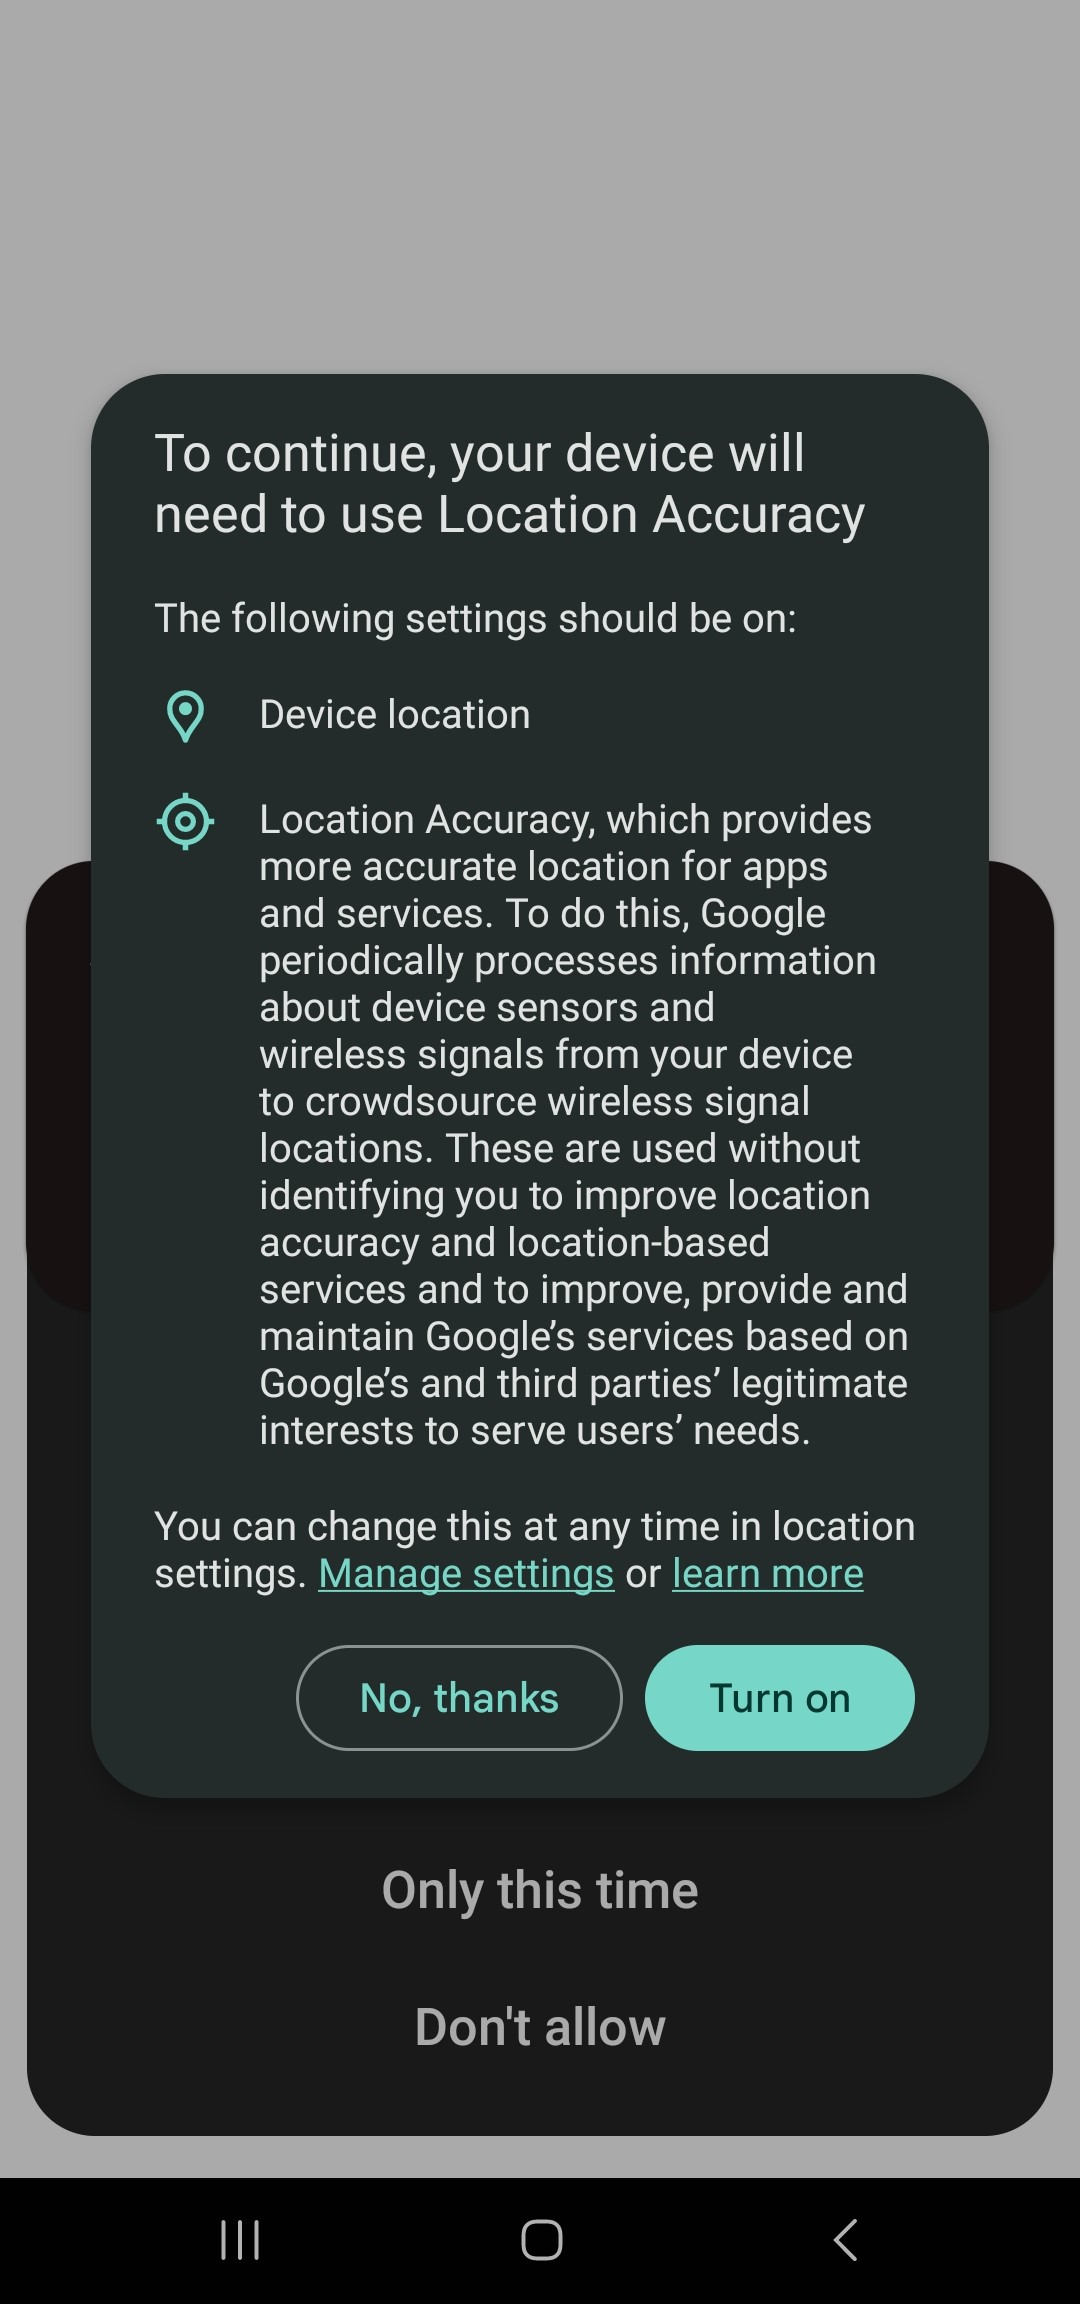
\includegraphics[width=0.4\textwidth]{images/permission-location-1.jpg} 
		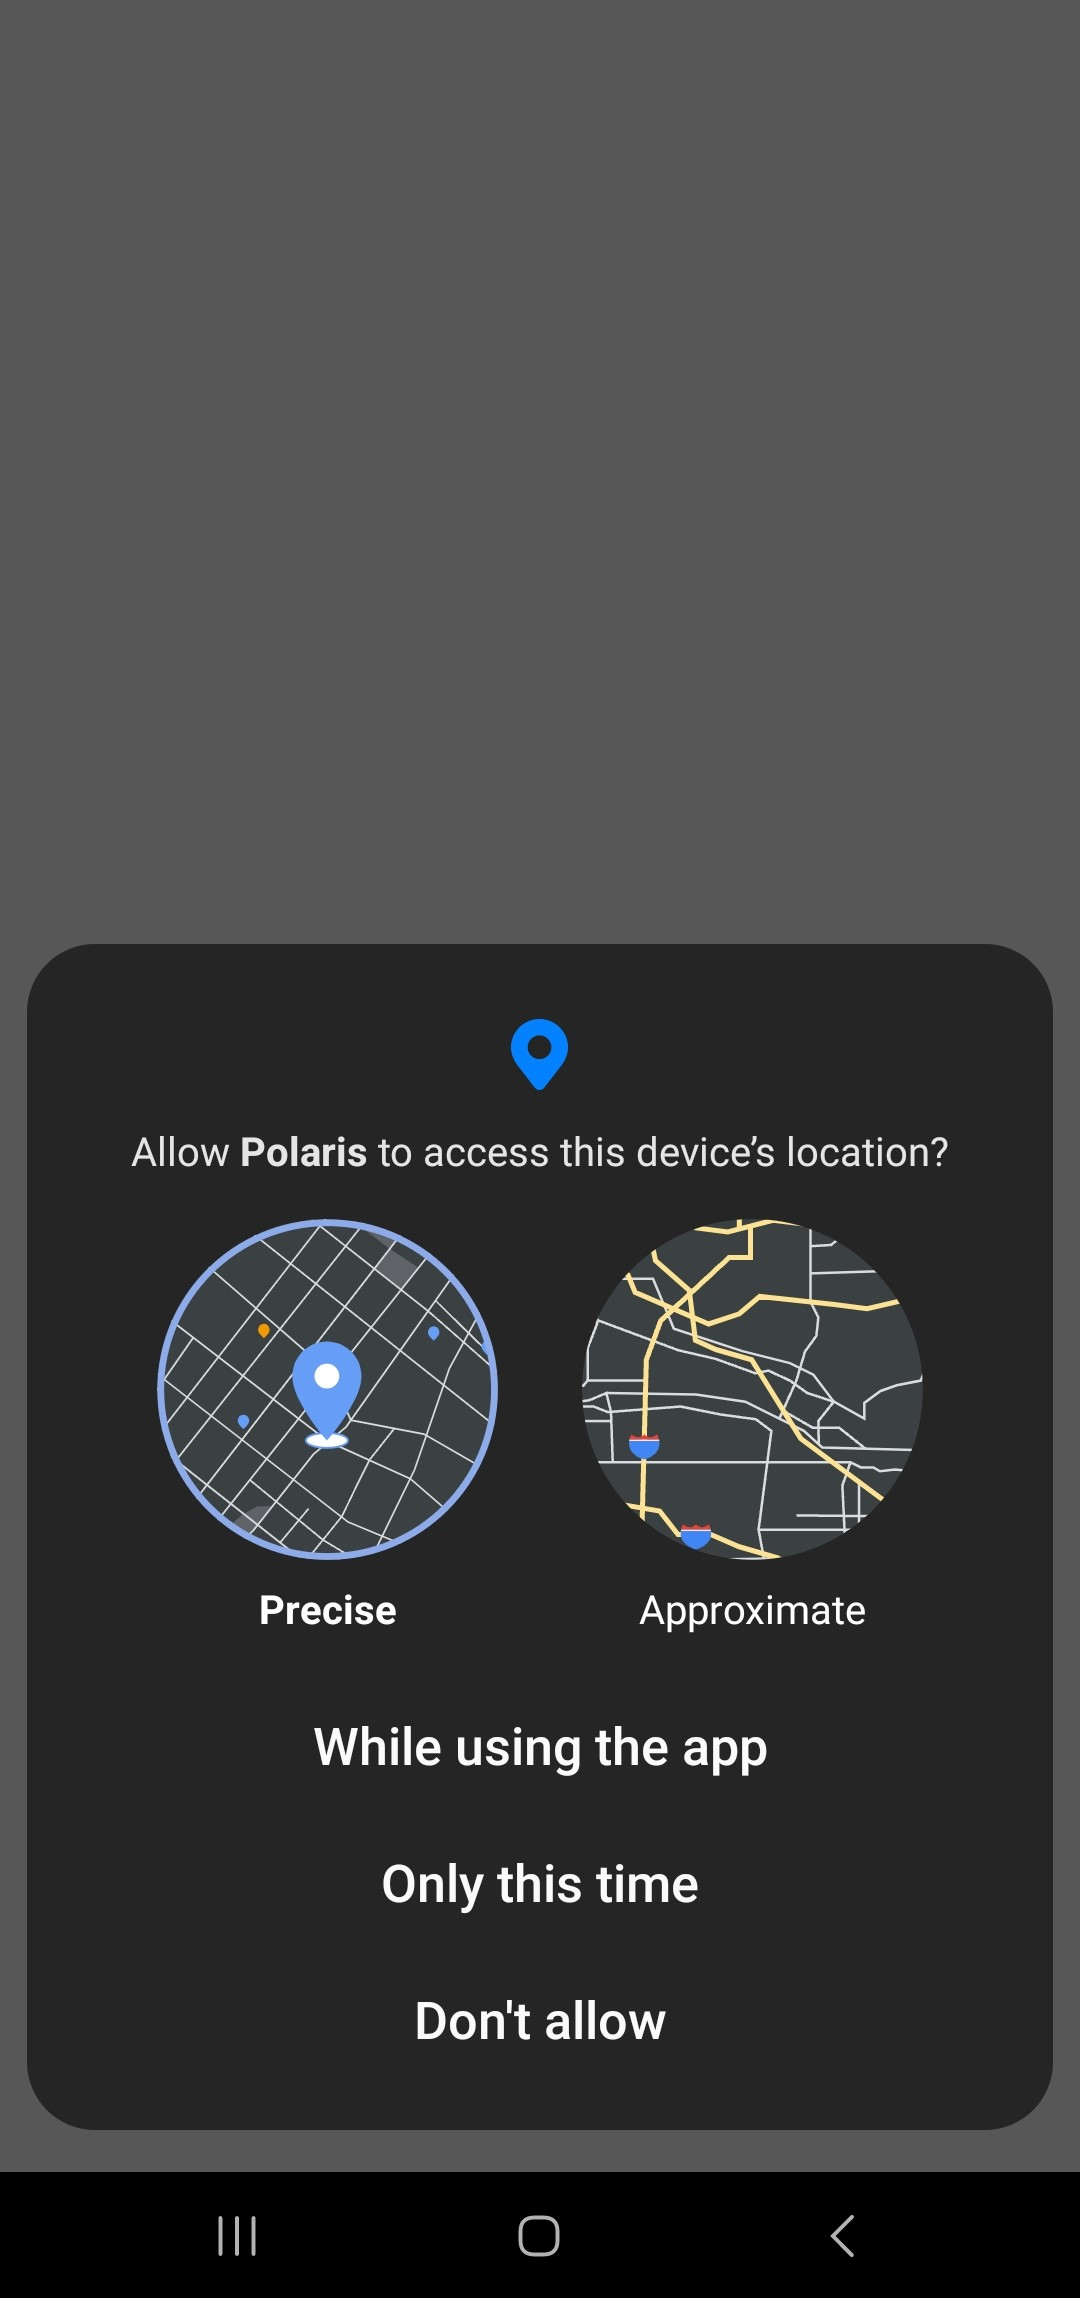
\includegraphics[width=0.4\textwidth]{images/permission-location-2.jpg} 
	\end{center}
	در دو مورد بالا که دسترسی به مکان‌یابی درخواست شده است، می‌بایست در  تصویر سمت راست \lr{Turn on} و در دسترسی درخواستی تصویر سمت چپ گزینه Precise و \lr{While using the app} را انتخاب نمود که برنامه بتواند به درستی کار کند. همچنین در دفعات بعدی ورود به برنامه برای صحت عملکرد فعالیت‌های background این برنامه دسترسی به مکان‌یابی مطابق زیر درخواست می‌شود:
	\begin{center}
		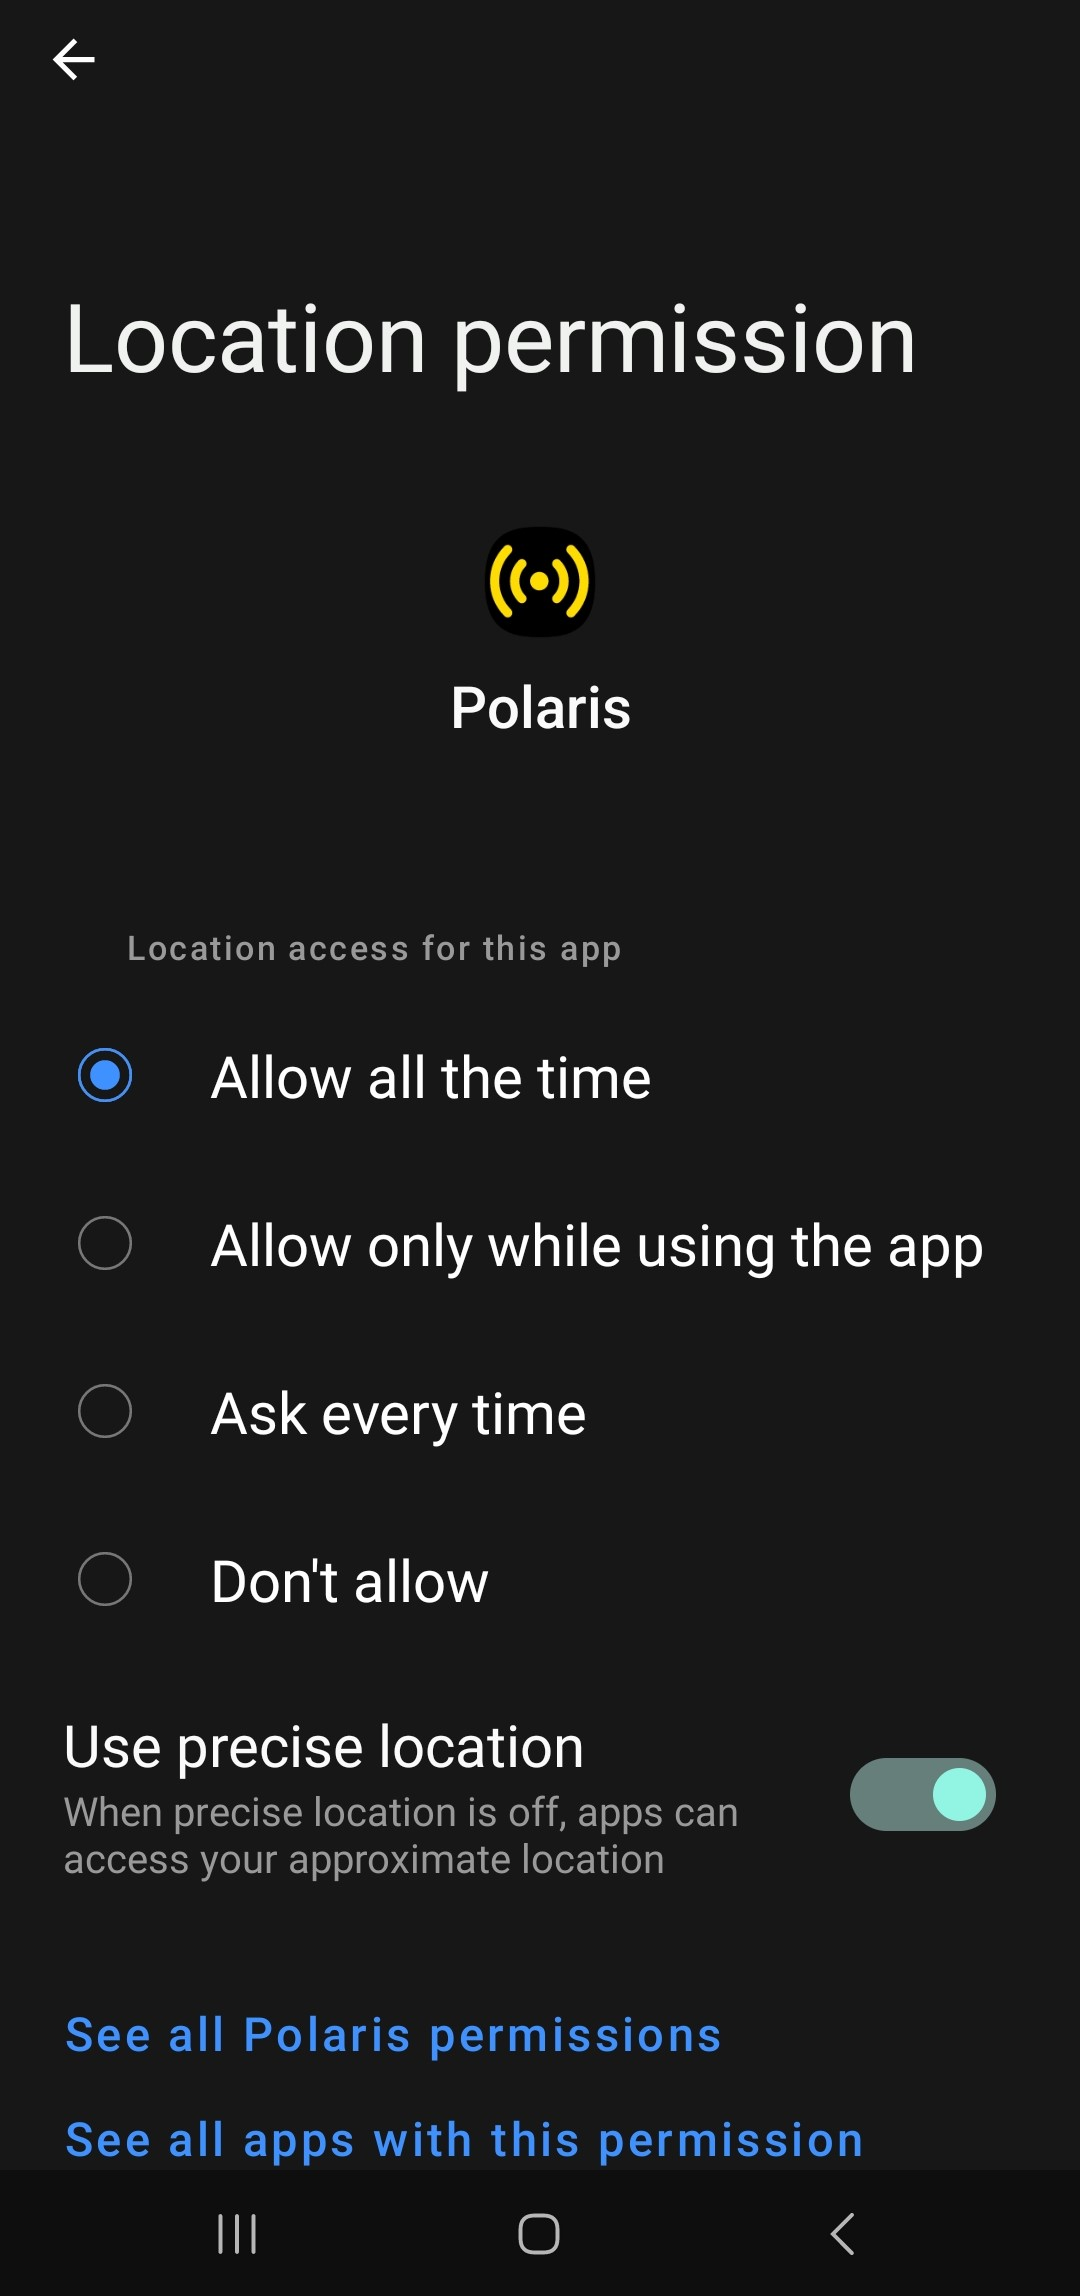
\includegraphics[width=0.4\textwidth]{images/permission-location-3.jpg} 
	\end{center}
	در این درخواست نیز طبق تصویر نیاز است که گزینه \lr{Allow all the time} انتخاب شود.
	در مرحله بعدی دسترسی‌های زیر درخواست می‌شوند:
	\begin{center}
		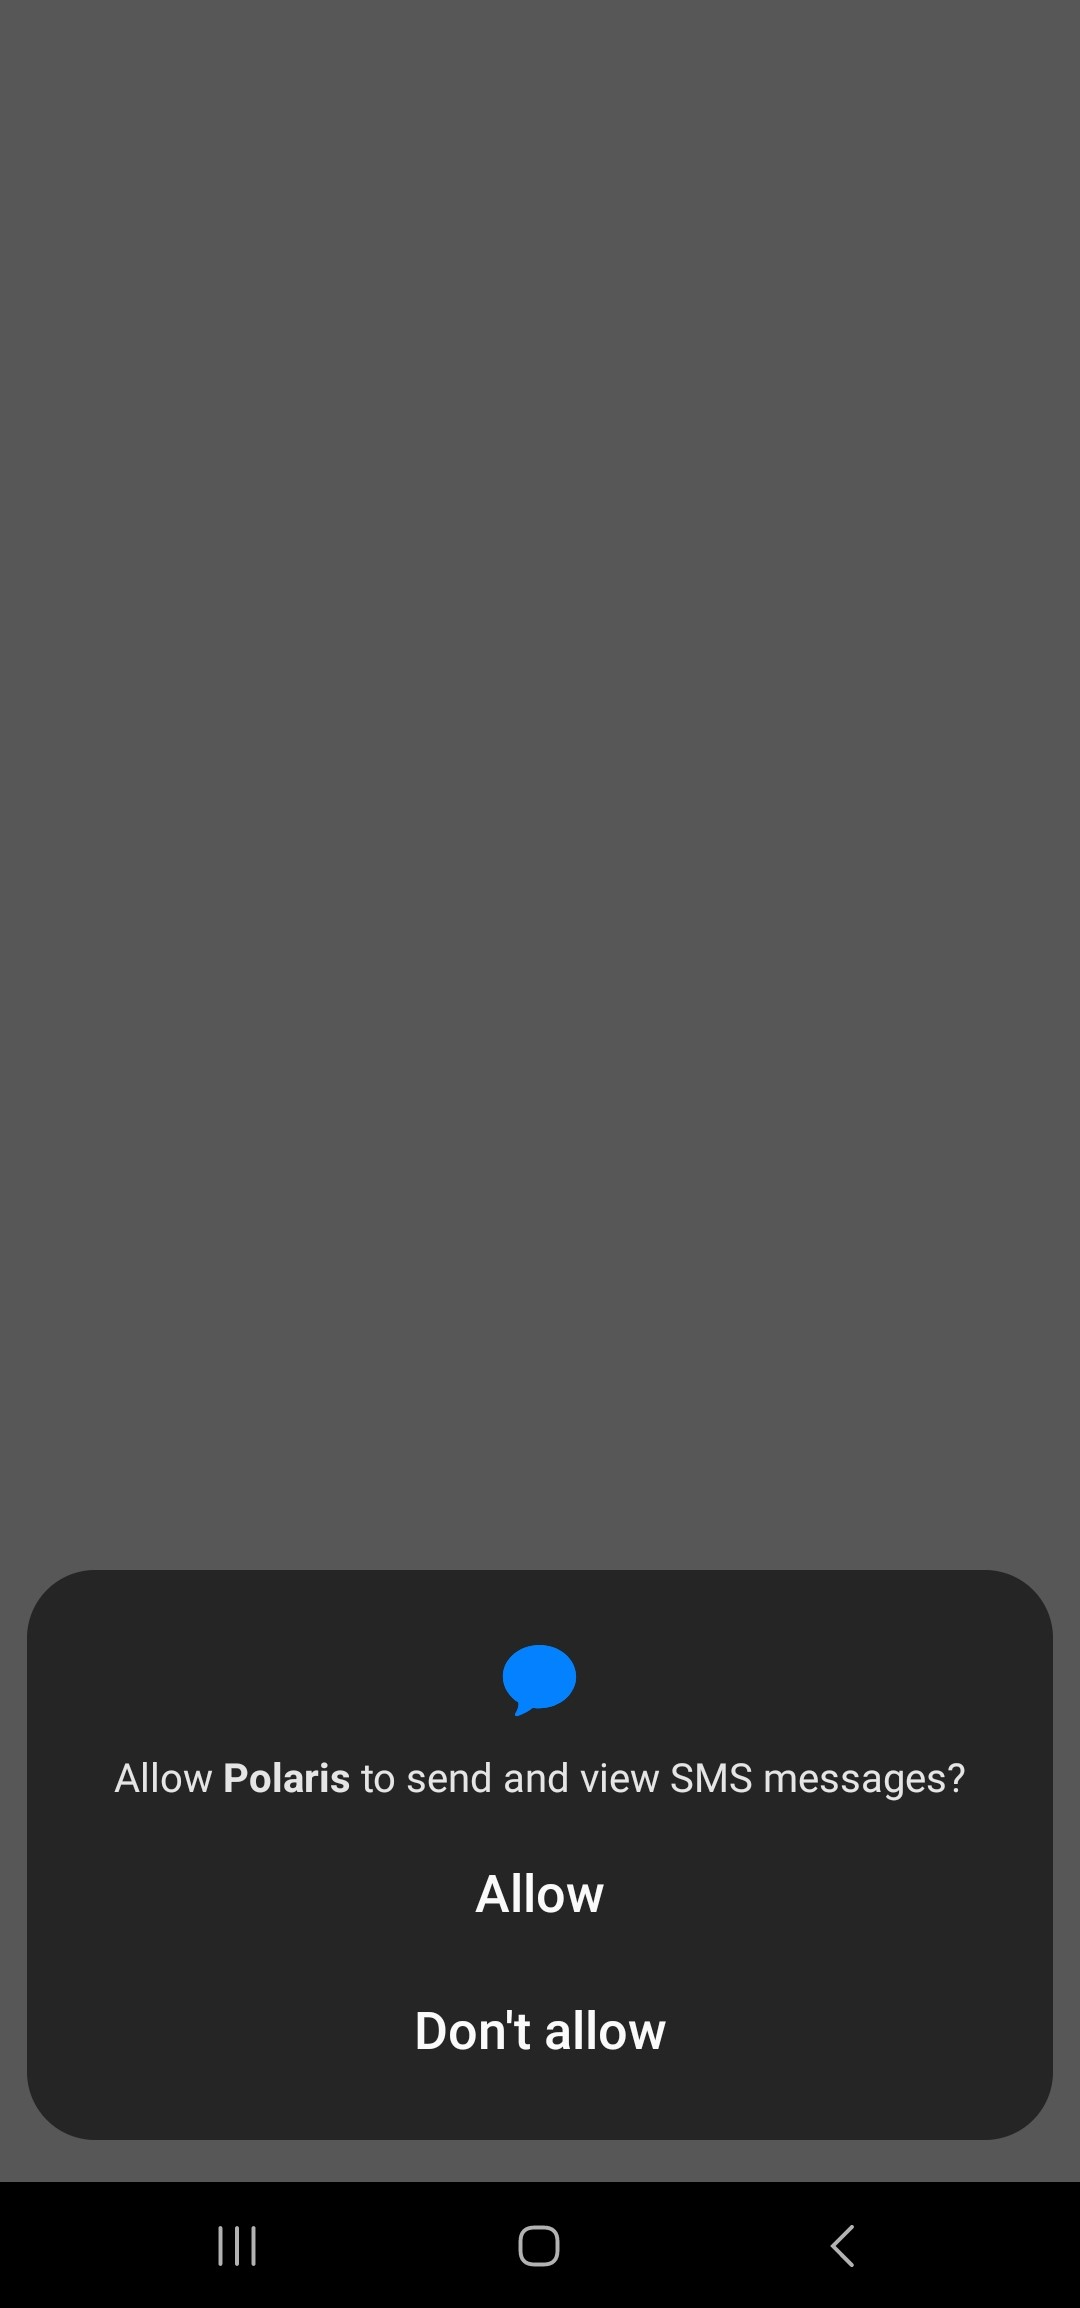
\includegraphics[width=0.4\textwidth]{images/permission-sms.jpg}
		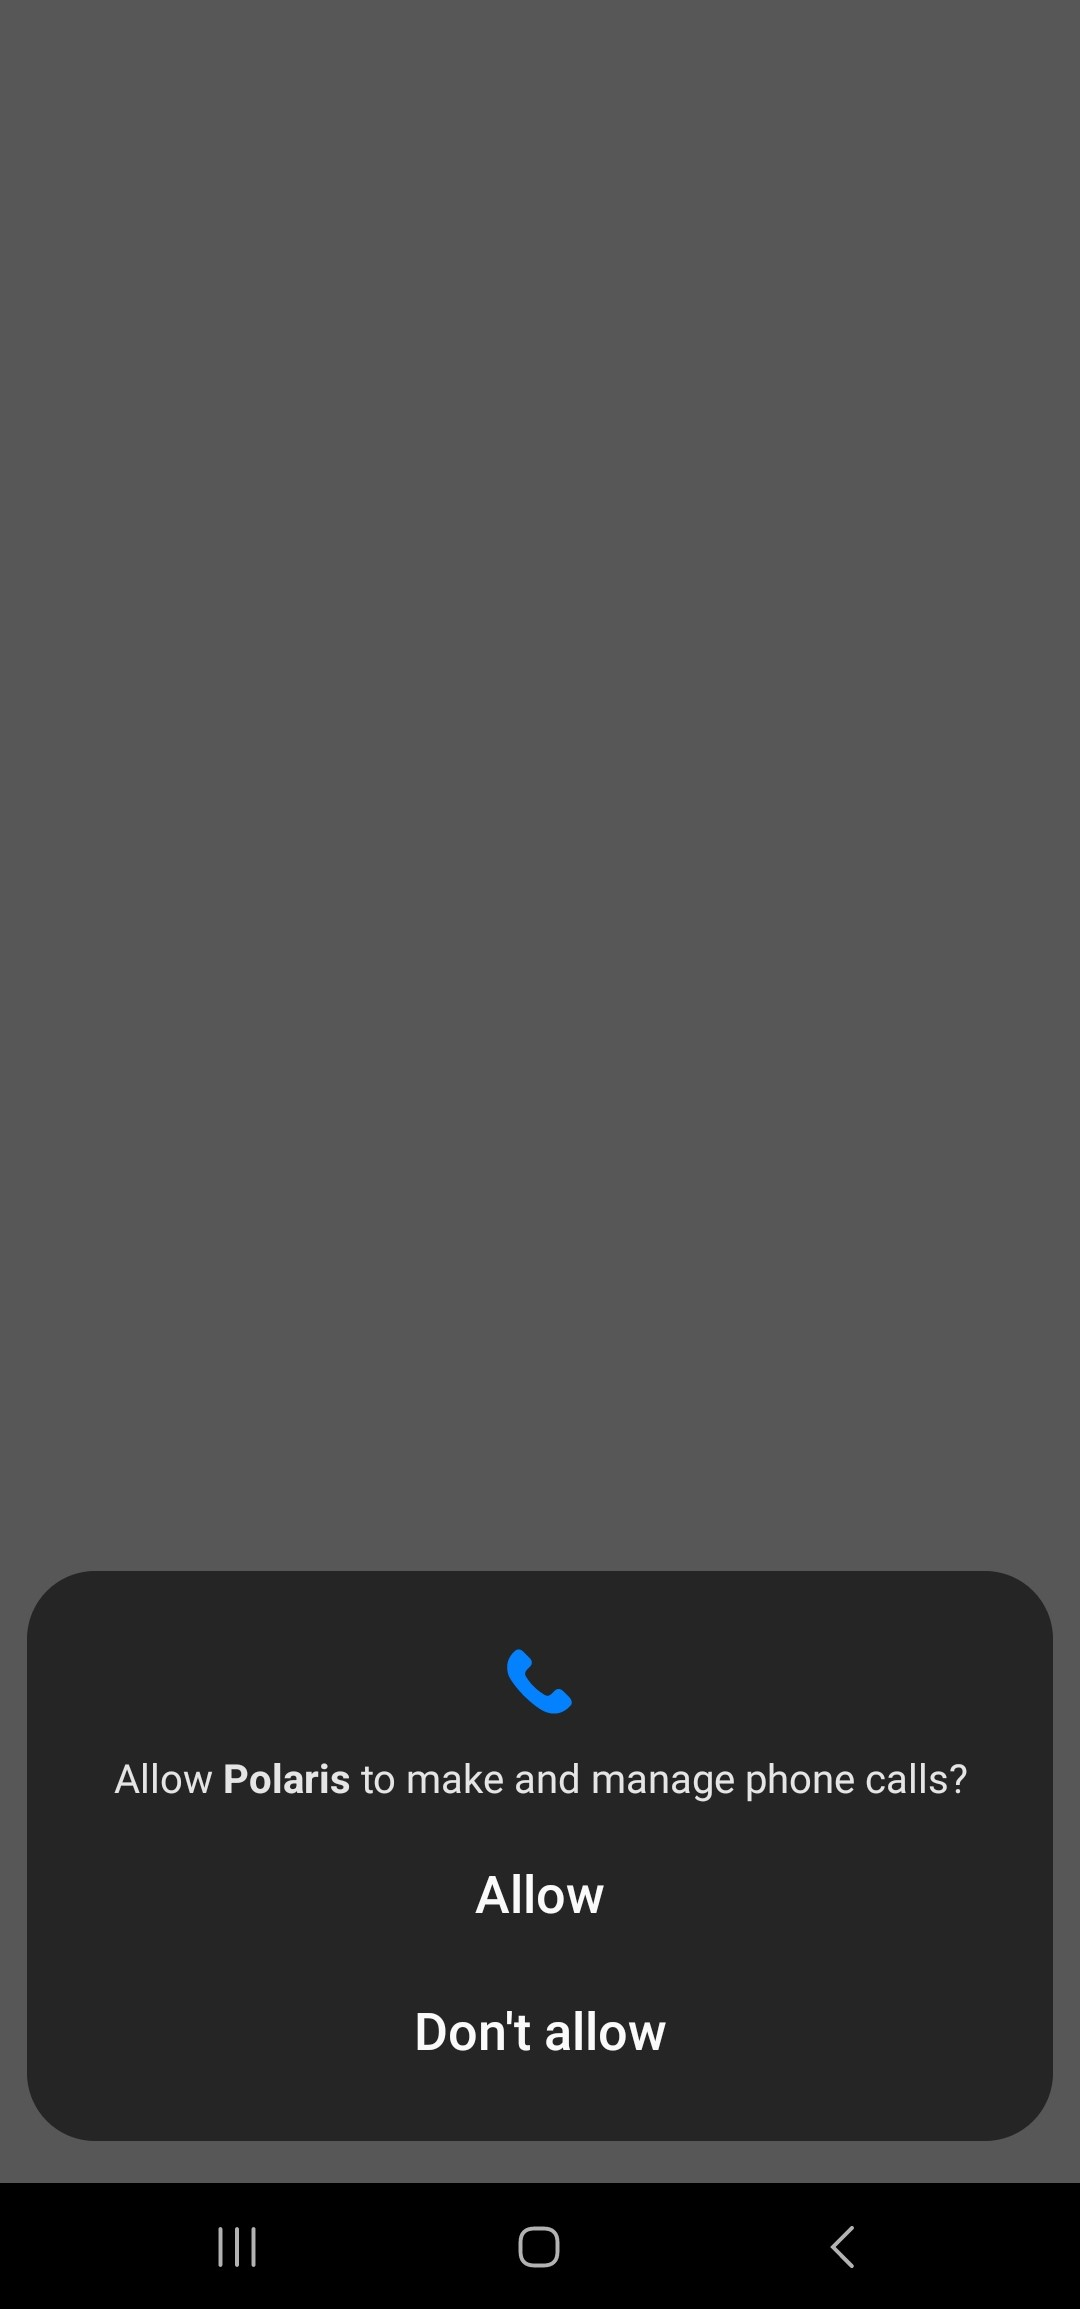
\includegraphics[width=0.4\textwidth]{images/permission-call.jpg}
	\end{center}
	
	
	این دو دسترسی مربوط به ارسال و خواندن پیامک و ایجاد و مدیریت تماس می‌باشند و نیاز است گزینه Allow انتخاب شود.
	در نهایت نیز دو دسترسی زیر درخواست می‌شود:
	\begin{center}
		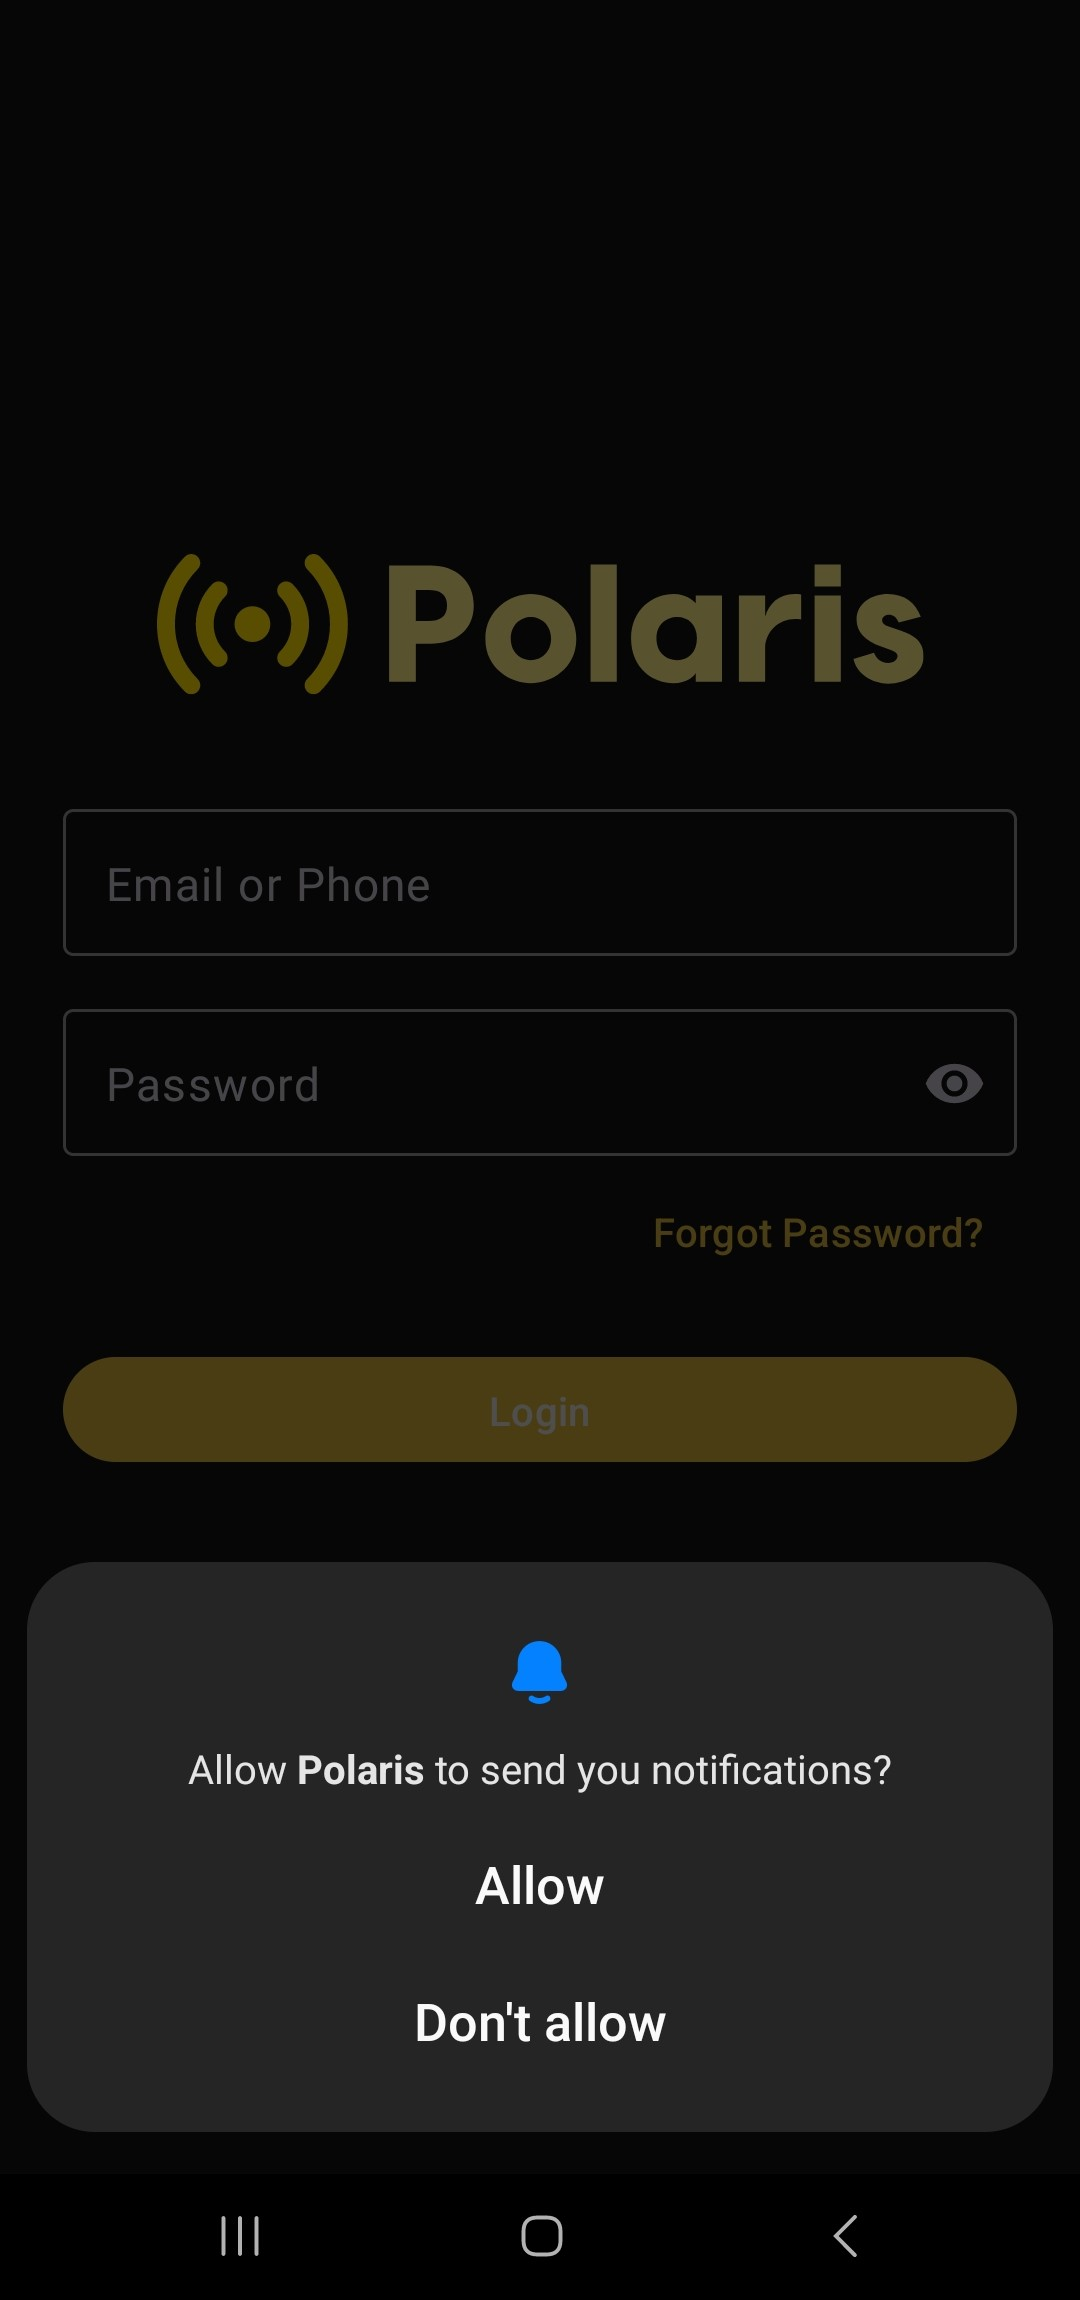
\includegraphics[width=0.4\textwidth]{images/permission-notification.jpg}
		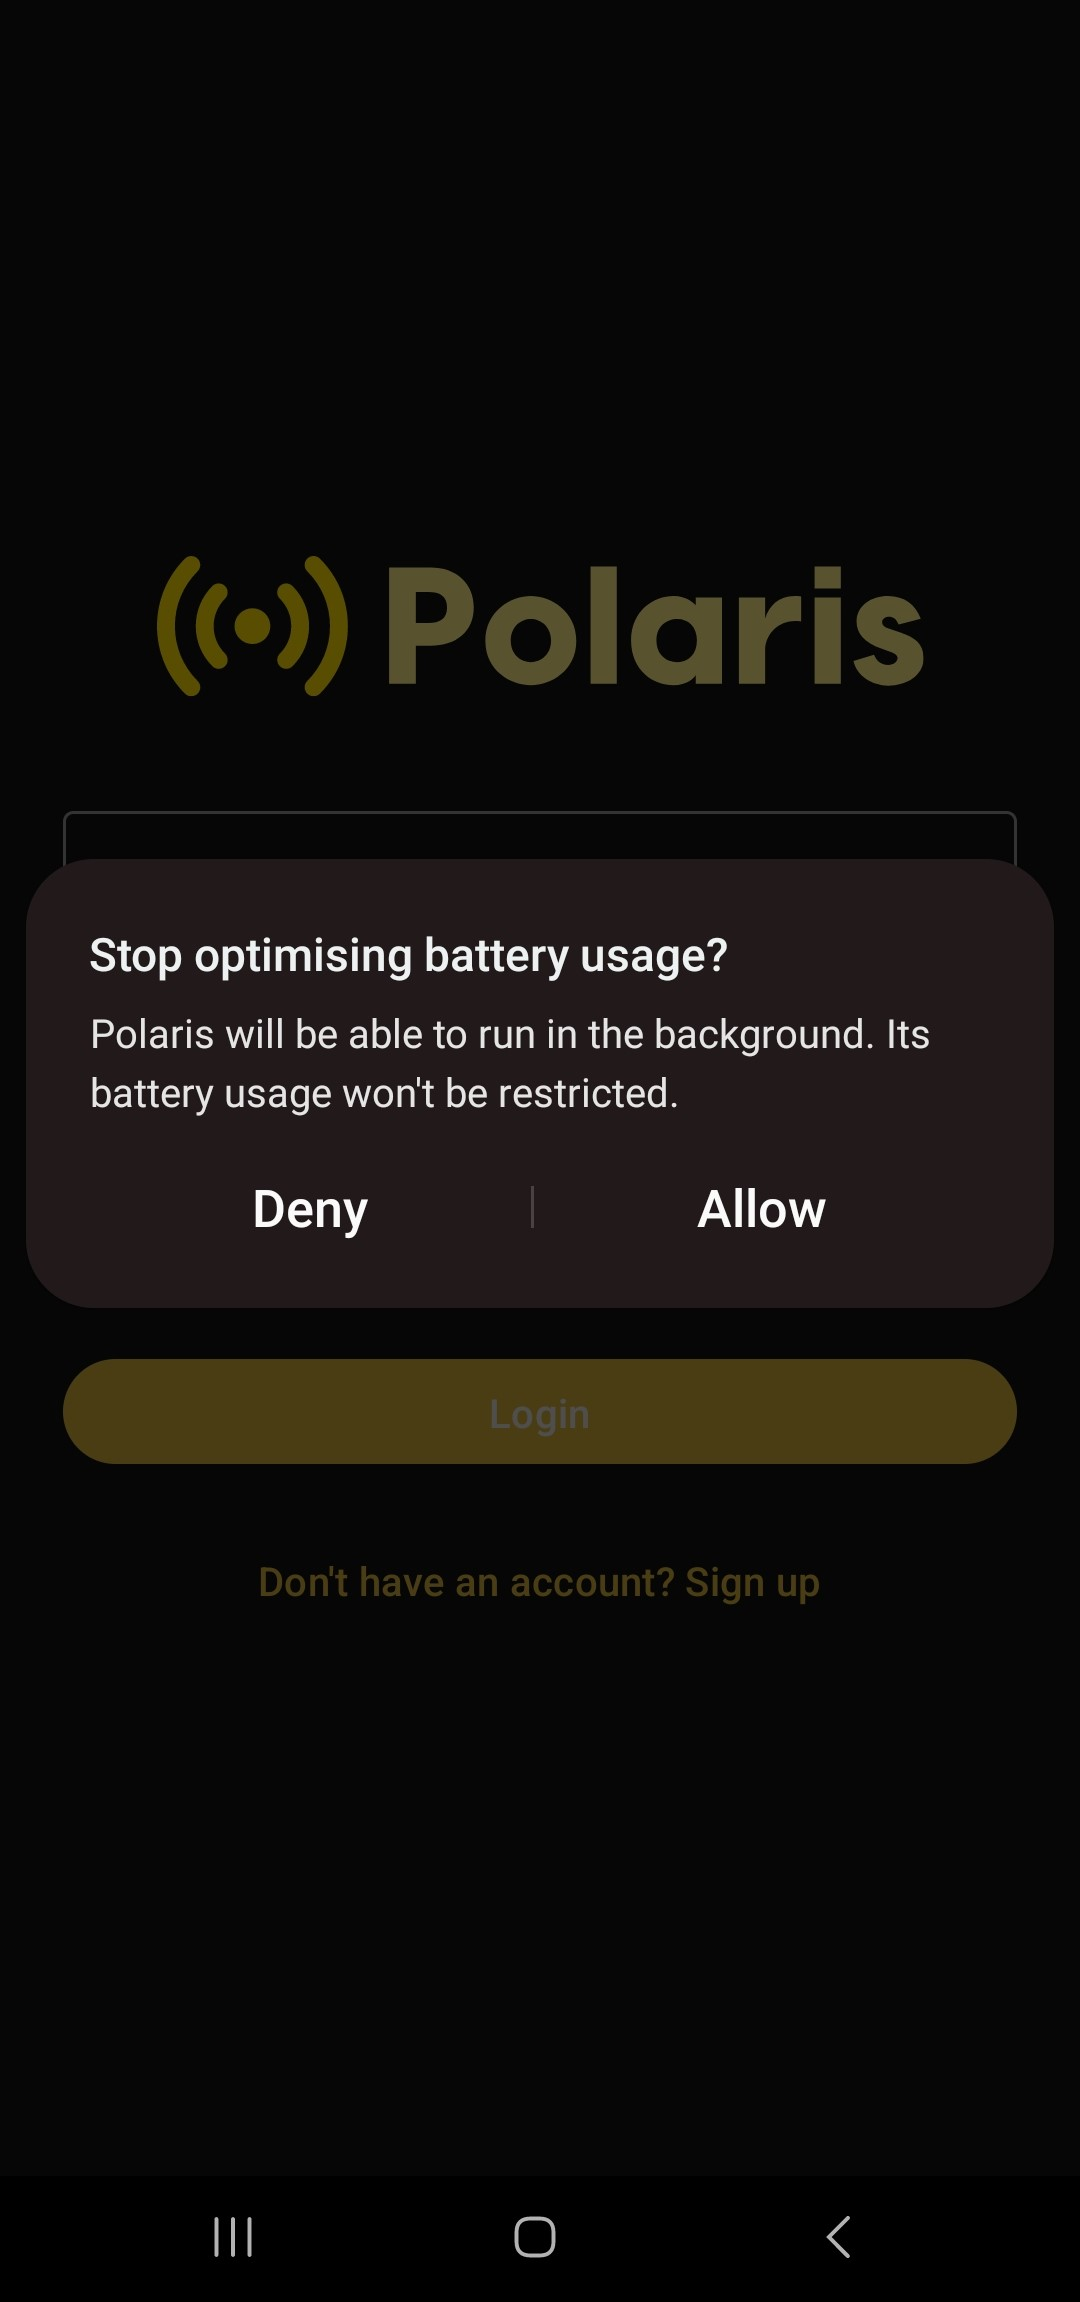
\includegraphics[width=0.4\textwidth]{images/permission-battery-optimization.jpg}
	\end{center}
	در دو دسترسی بالا نیز نیاز است که گزینه Allow انتخاب شود که فعالیت background برنامه به صورت صحیح صورت گیرد.
	در انتها نیز با صفحه زیر مواجه می‌شویم:
	\begin{center}
		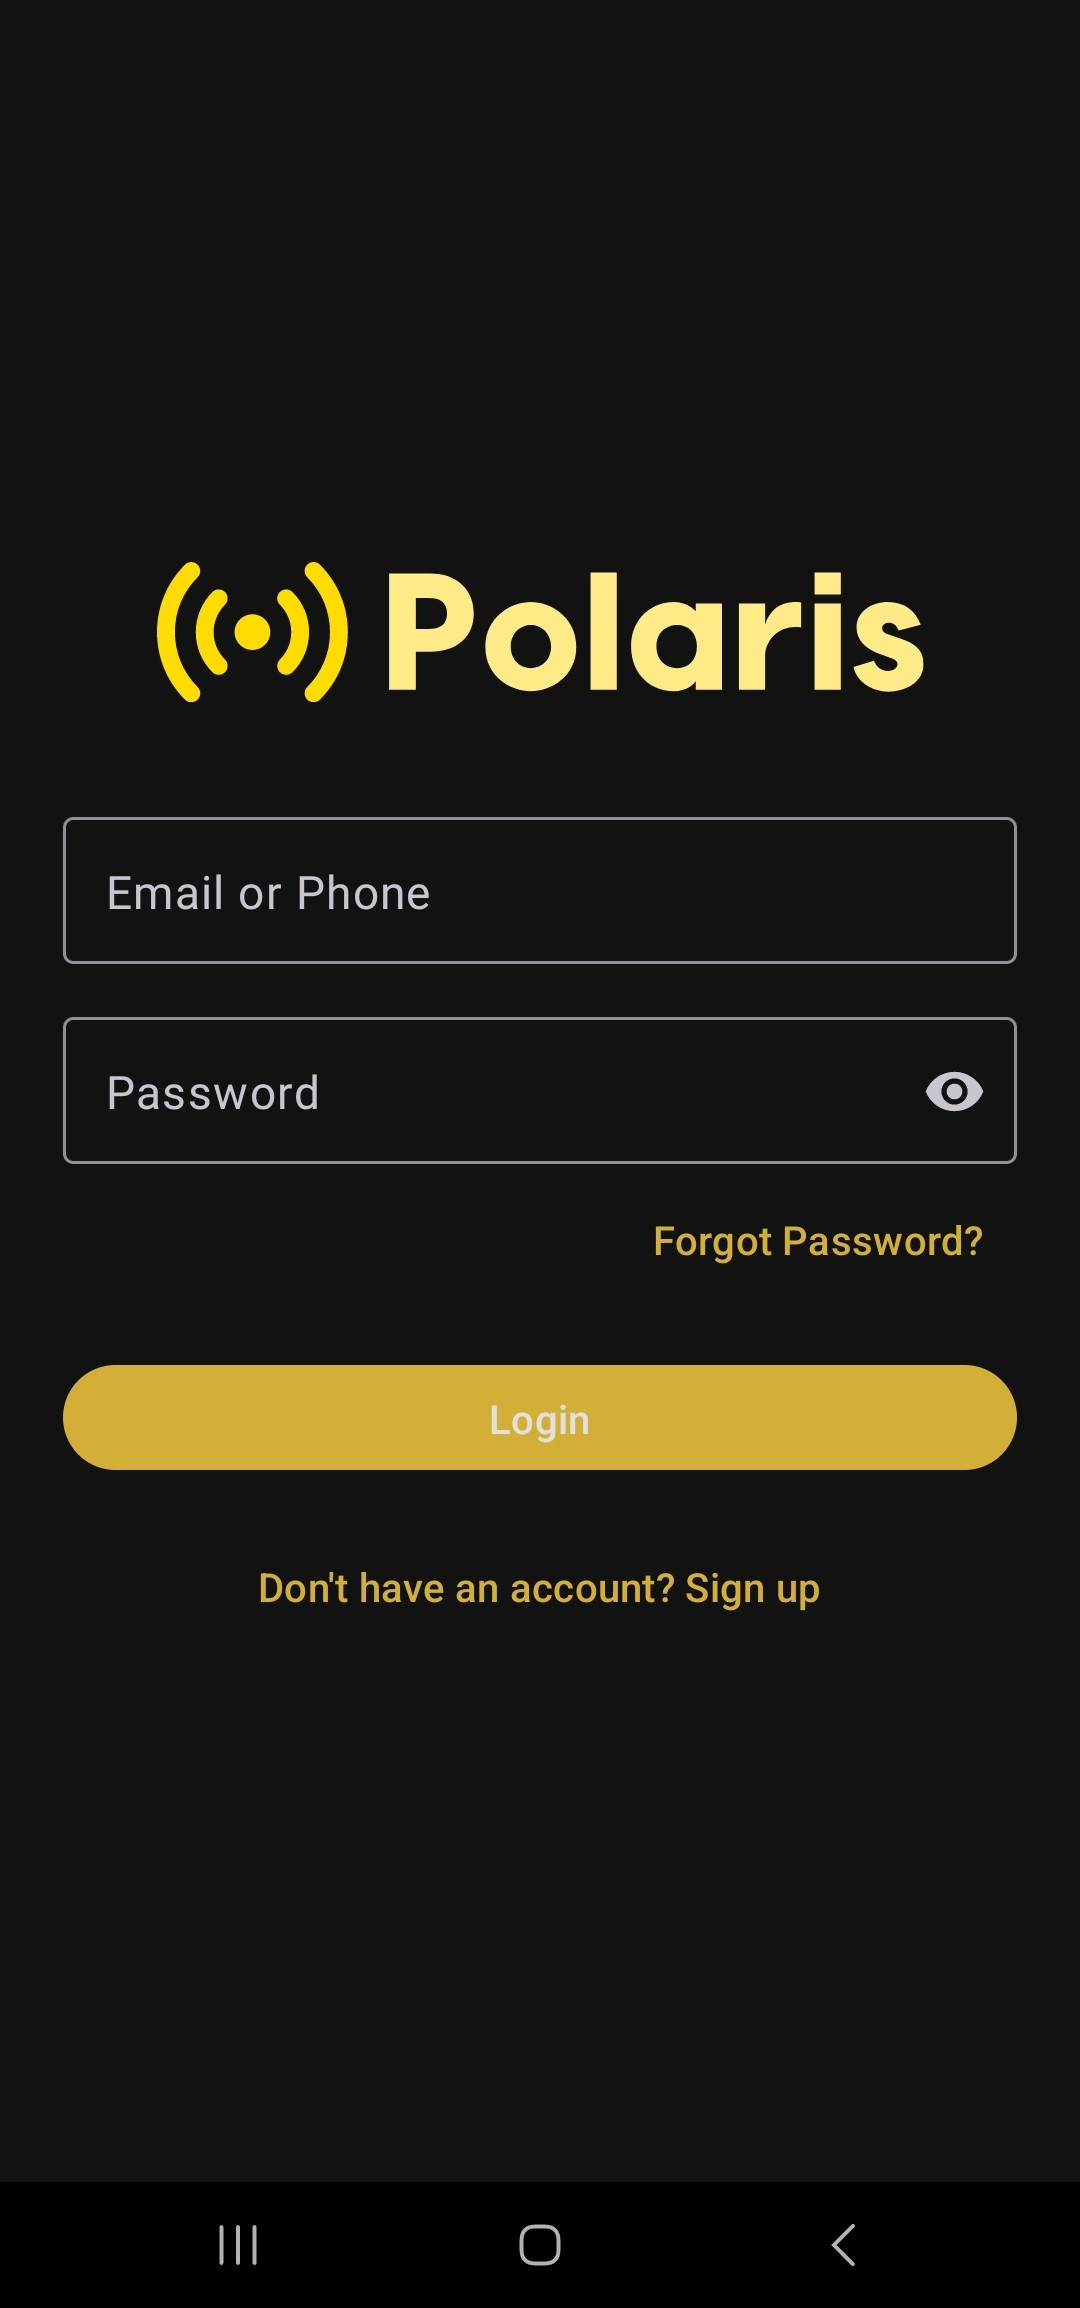
\includegraphics[width=0.4\textwidth]{images/login-empty.jpg}
	\end{center}
\end{itemize}
\section{مدیریت حساب کاربری}
\begin{itemize}
	\item  ثبت نام: برای ثبت نام در این برنامه نیاز است که ابتدا در صفحه Login که صفحه ابتدایی برنامه پس از دادن دسترسی‌های گفته شده است لینک \lr{Don't have an account?Sign up} را انتخاب کرده تا به صفحه زیر منتقل شوید:
	\begin{center}
		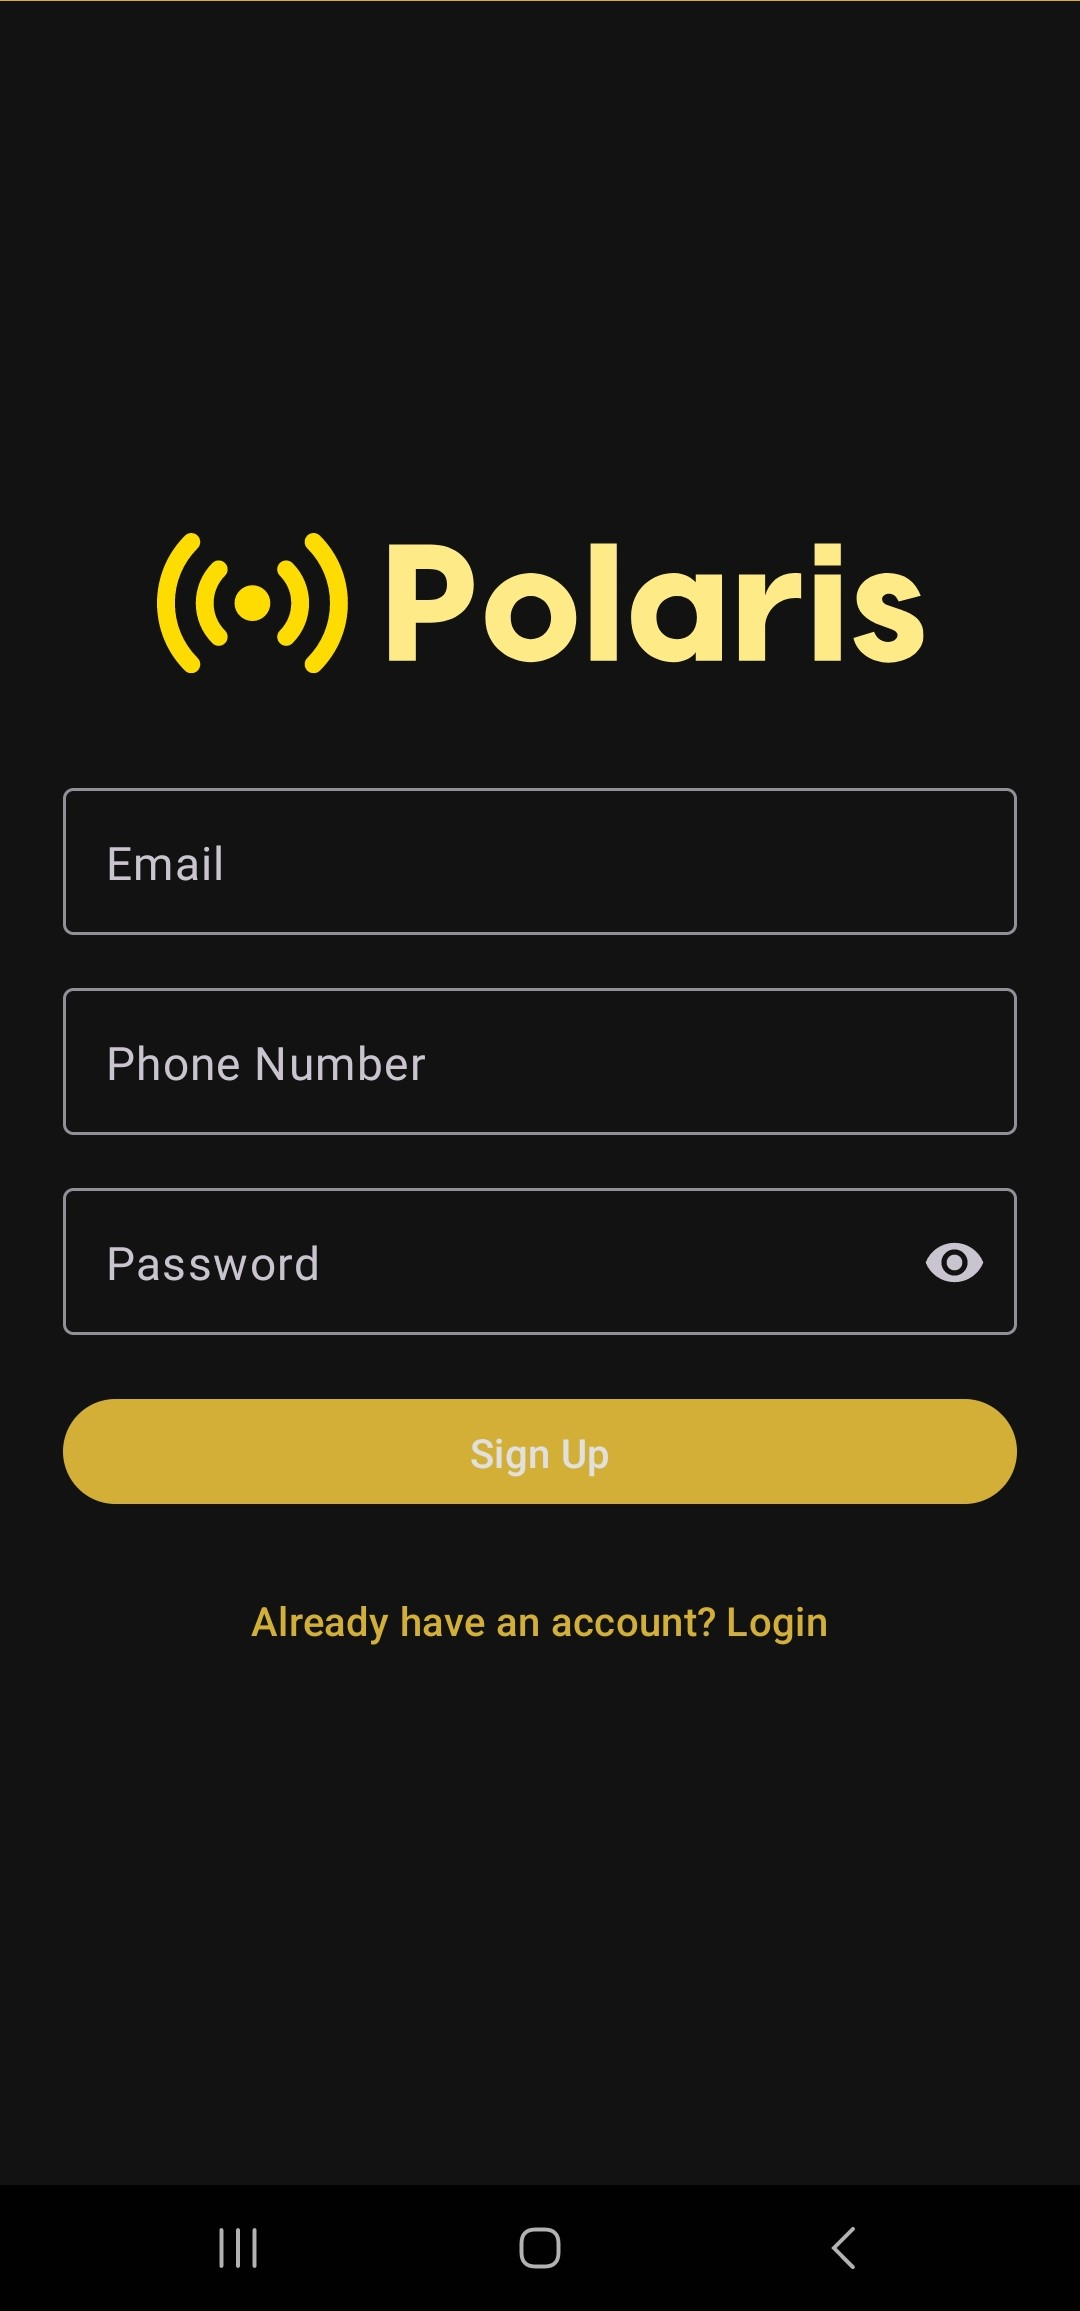
\includegraphics[width=0.4\textwidth]{images/signup-empty.jpg}
	\end{center}
	\begin{itemize}
		\item پر کردن فرم ثبت نام:
		در این صفحه همانطور که در هر قسمت اطلاعات خود را که شامل پست الکترونیک، شماره تلفن همراه و گذرواژه می‌باشد را وارد کنید. لازم به ذکر است که شماره تلفن همراه می‌بایست به شکل 09xxxxxxxxx وارد شود و گذرواژه می‌بایست حداقل 8 کاراکتر(اعم از عدد و حروف الفبا) باشد. پس از وارد کردن مشخصات بر روی دکمه \lr{Sign Up} کلیک کرده و در صورت با شکست مواجه شدن درخواست خطای مربوطه نمایش داده شده و در غیر این صورت با موفقیت آمیز بودن ایجاد حساب به مرحله بعد می‌رویم.

		\item  تأیید آدرس ایمیل: پس از وارد کردن مشخصات کاربر در \lr{Sign Up} به صفحه زیر وارد می‌شویم:
			\begin{center}
				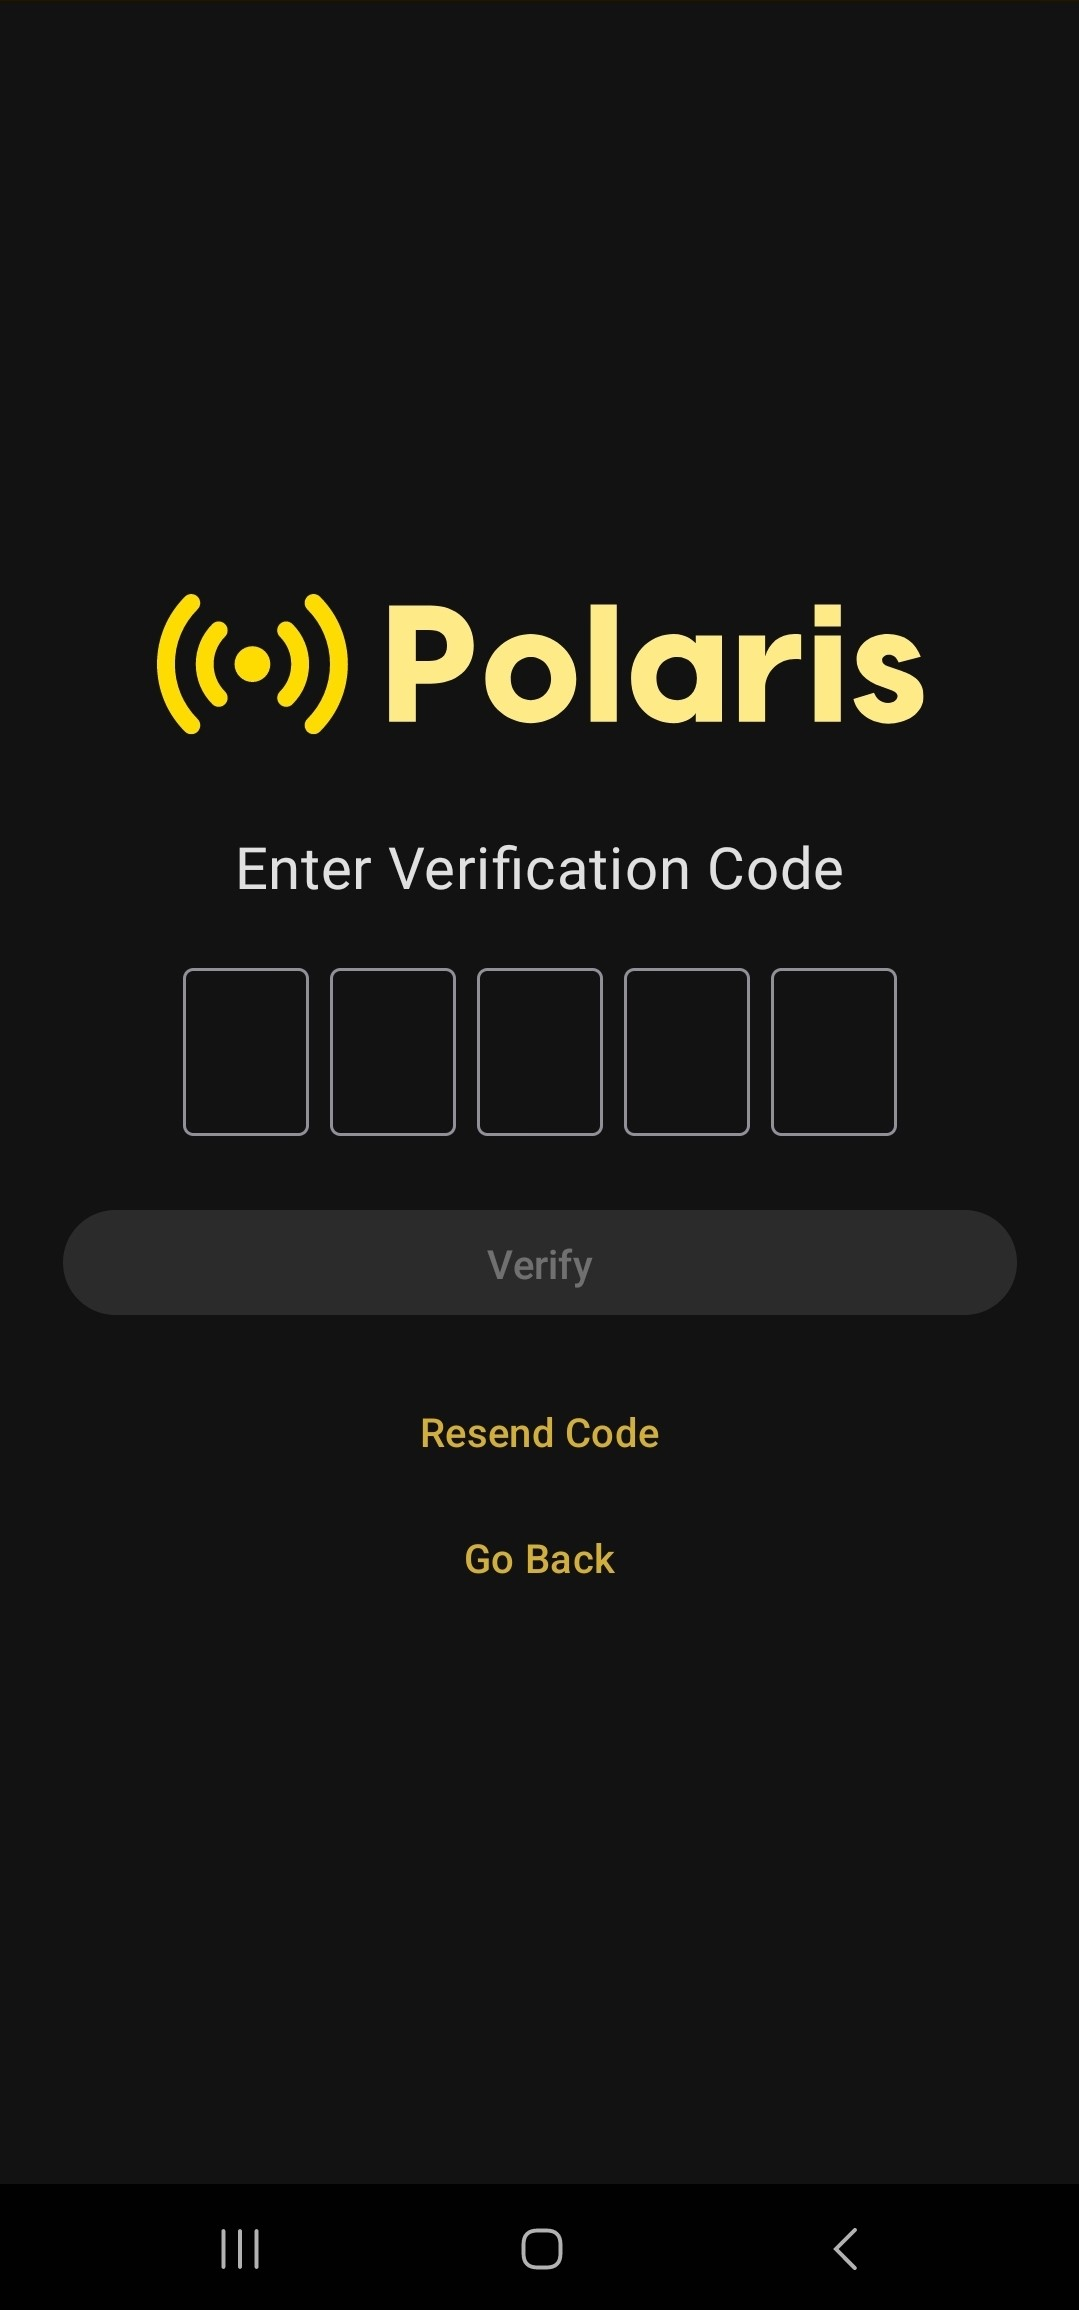
\includegraphics[width=0.4\textwidth]{images/verify-empty.jpg}
			\end{center}
		در این قسمت نیاز است رمز 5 رقمی که به ایمیلی در مرحله پیشین وارد کرده اید ارسال شده است را وارد کنید. در این صفحه می‌توانید در صورت عدم دریافت کد بر روی لینک \lr{Resend Code} کلیک کنید تا کد مجدد برای شما ارسال شود. همچنین می‌توانید با انتخاب \lr{Go Back} به مرحله پیشین یعنی \lr{Sign Up} بازگردید. با وارد کردن کد ارسال شده پیام موفقیت آمیز بودن ایجاد حساب به صورت زیر نمایش داده می‌شود:
		\begin{center}
			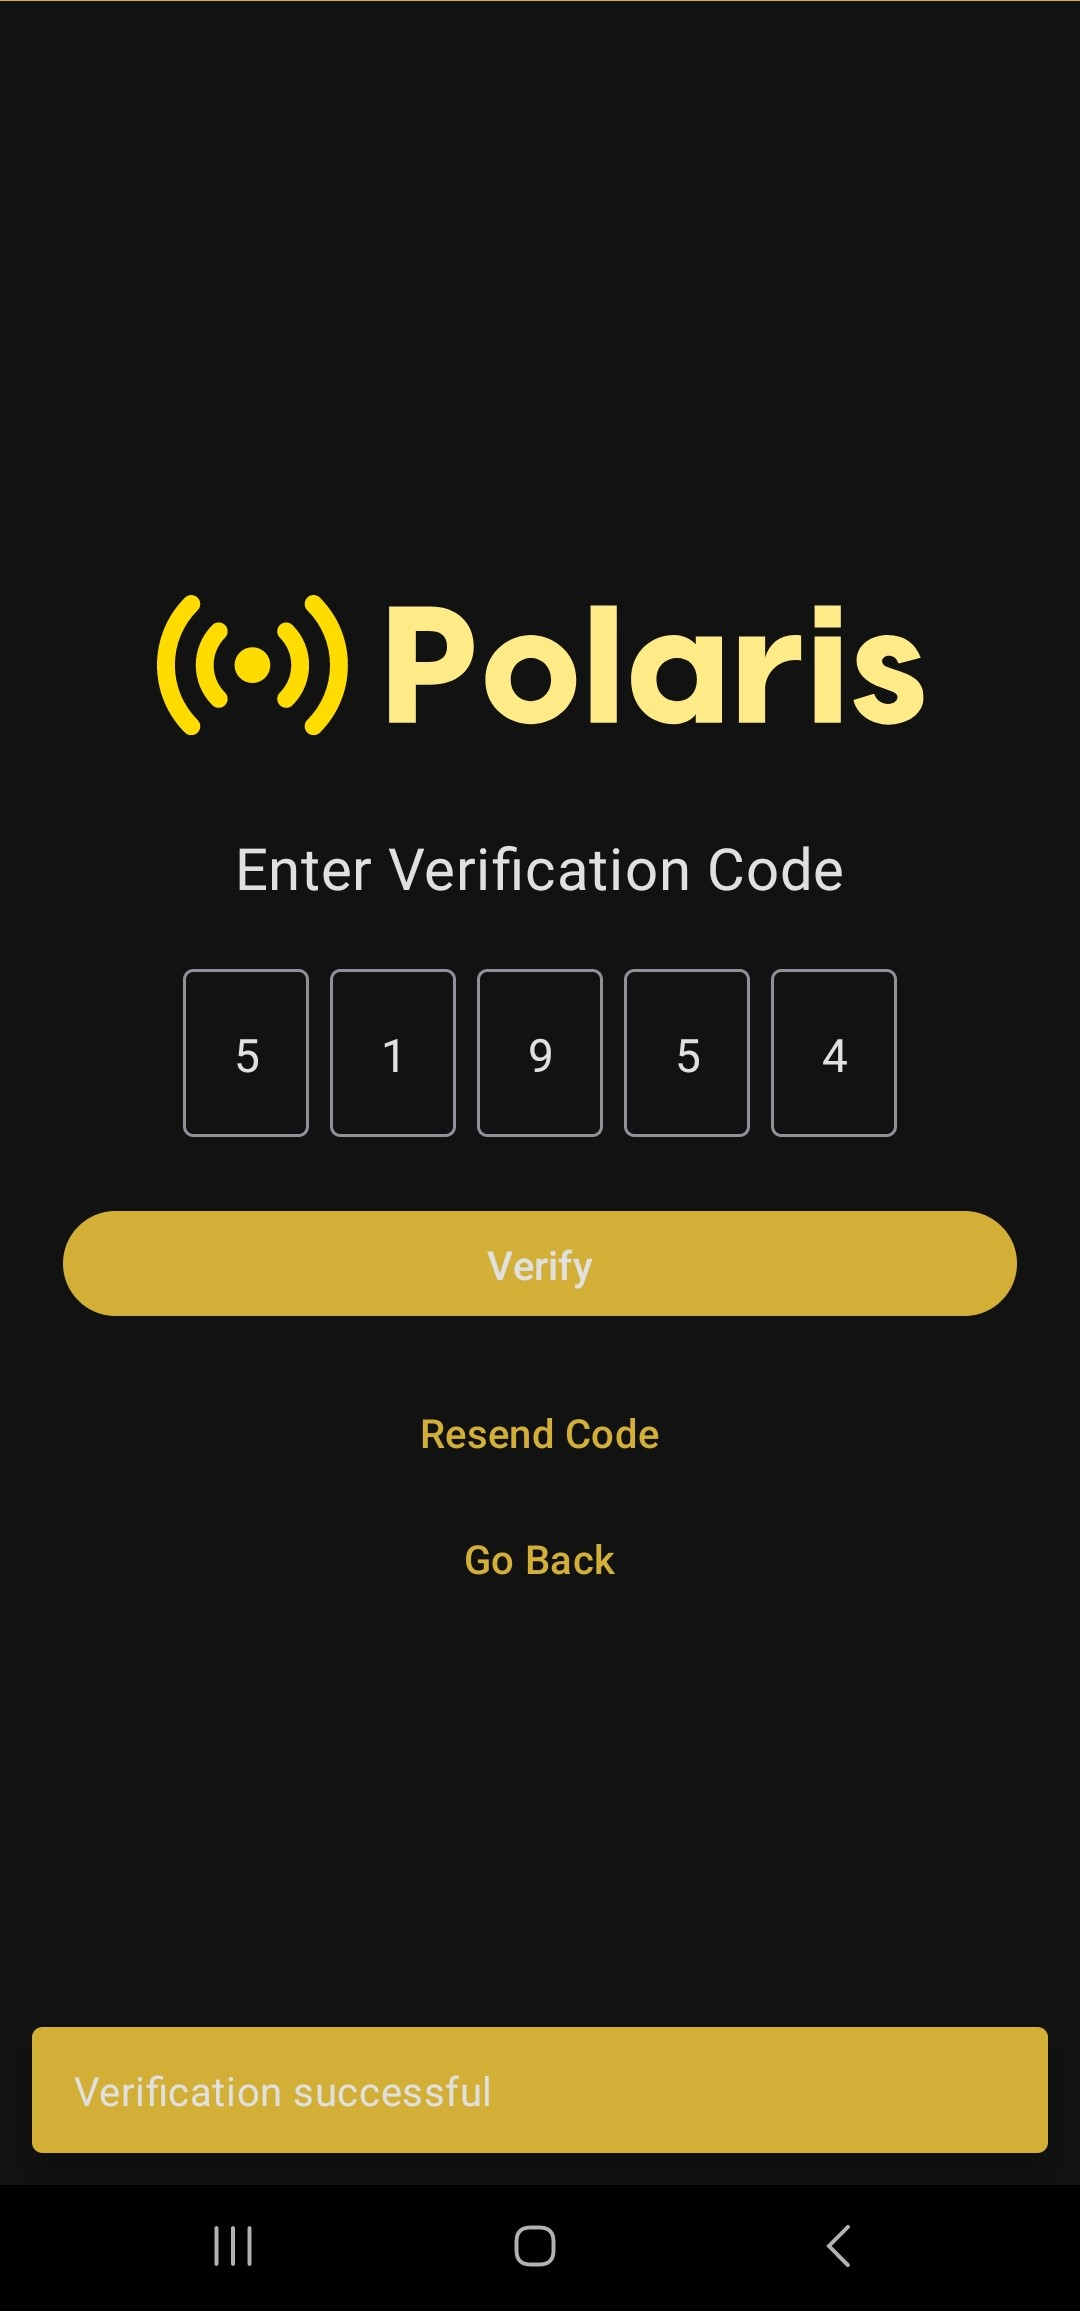
\includegraphics[width=0.4\textwidth]{images/verify-success.jpg}
		\end{center}
		پس از مشاهده این صفحه با یک تاخیر کوتاه به صفحه خانه هدایت می‌شوید که به دلیل عدم اندازه‌گیری قبلی به صورت زیر است:
		\begin{center}
			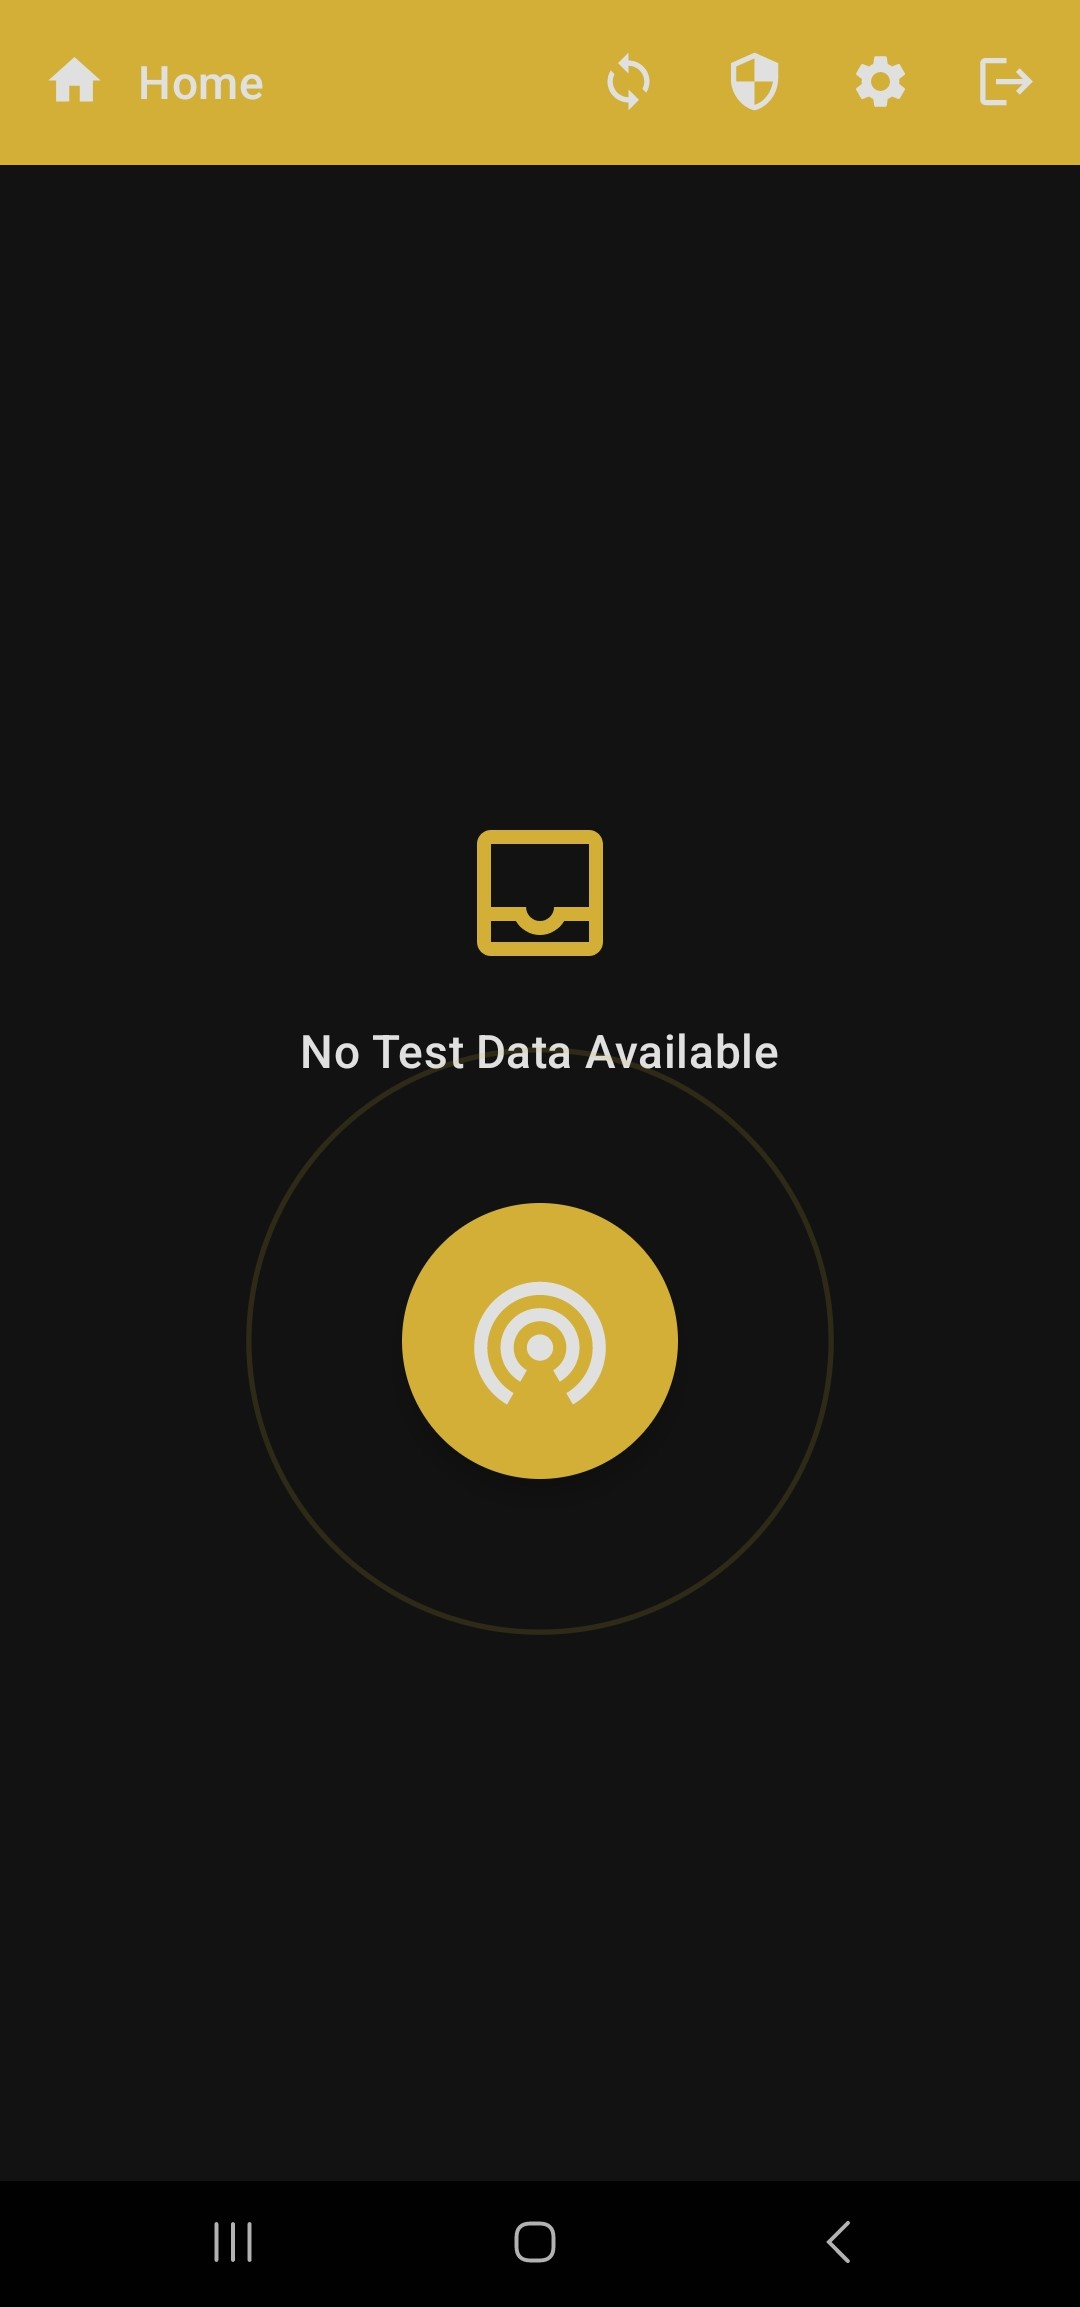
\includegraphics[width=0.4\textwidth]{images/home-empty.jpg}
		\end{center}
	\end{itemize}
	\item  ورود به حساب: در صفحه ابتدایی برنامه پس از وارد کردن مشخصات کاربری و کلیک بر روی دکمه Login در صورت با خطا مواجه شدن پیام خطای مناسب نمایش داده می‌شود و در صورت عدم تایید ایمیل به صفحه تایید ایمیل منتقل می‌شوید. در صورت موفقیت آمیز بودن این درخواست پیام موفقیت آمیز بودن به شکل زیر نمایش داده می‌شود:
		\begin{center}
			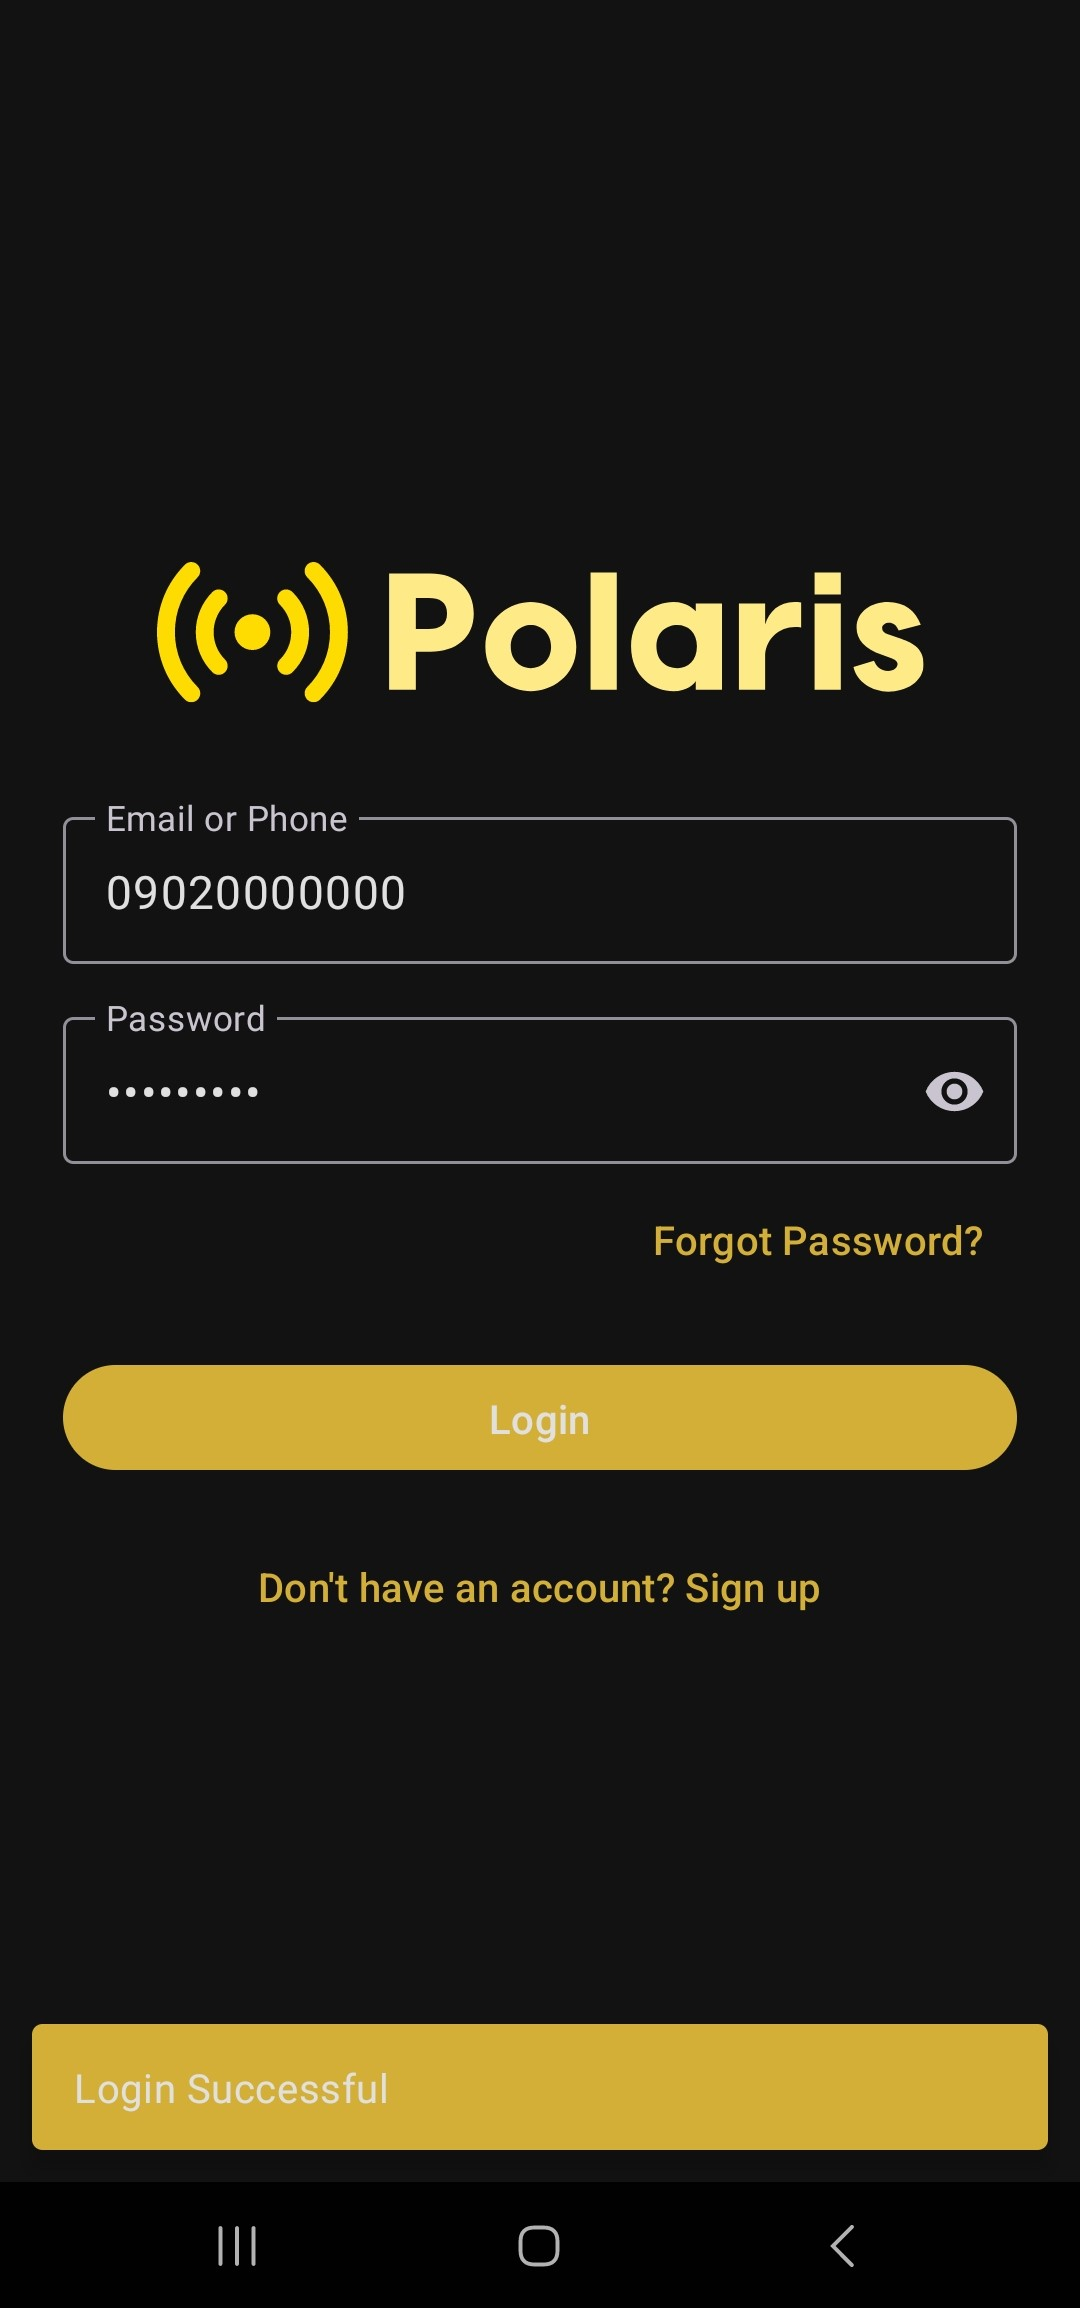
\includegraphics[width=0.4\textwidth]{images/login-success.jpg}
		\end{center}
		سپس بعد از کمی تاخیر به صفحه خانه منتقل می‌شوید که در صورت داشتن اندازه‌گیری پیشین به صورت تصویر راست و در صورت عدم داشتن این داده‌ها به صورت تصویر چپ است:
		\begin{center}
			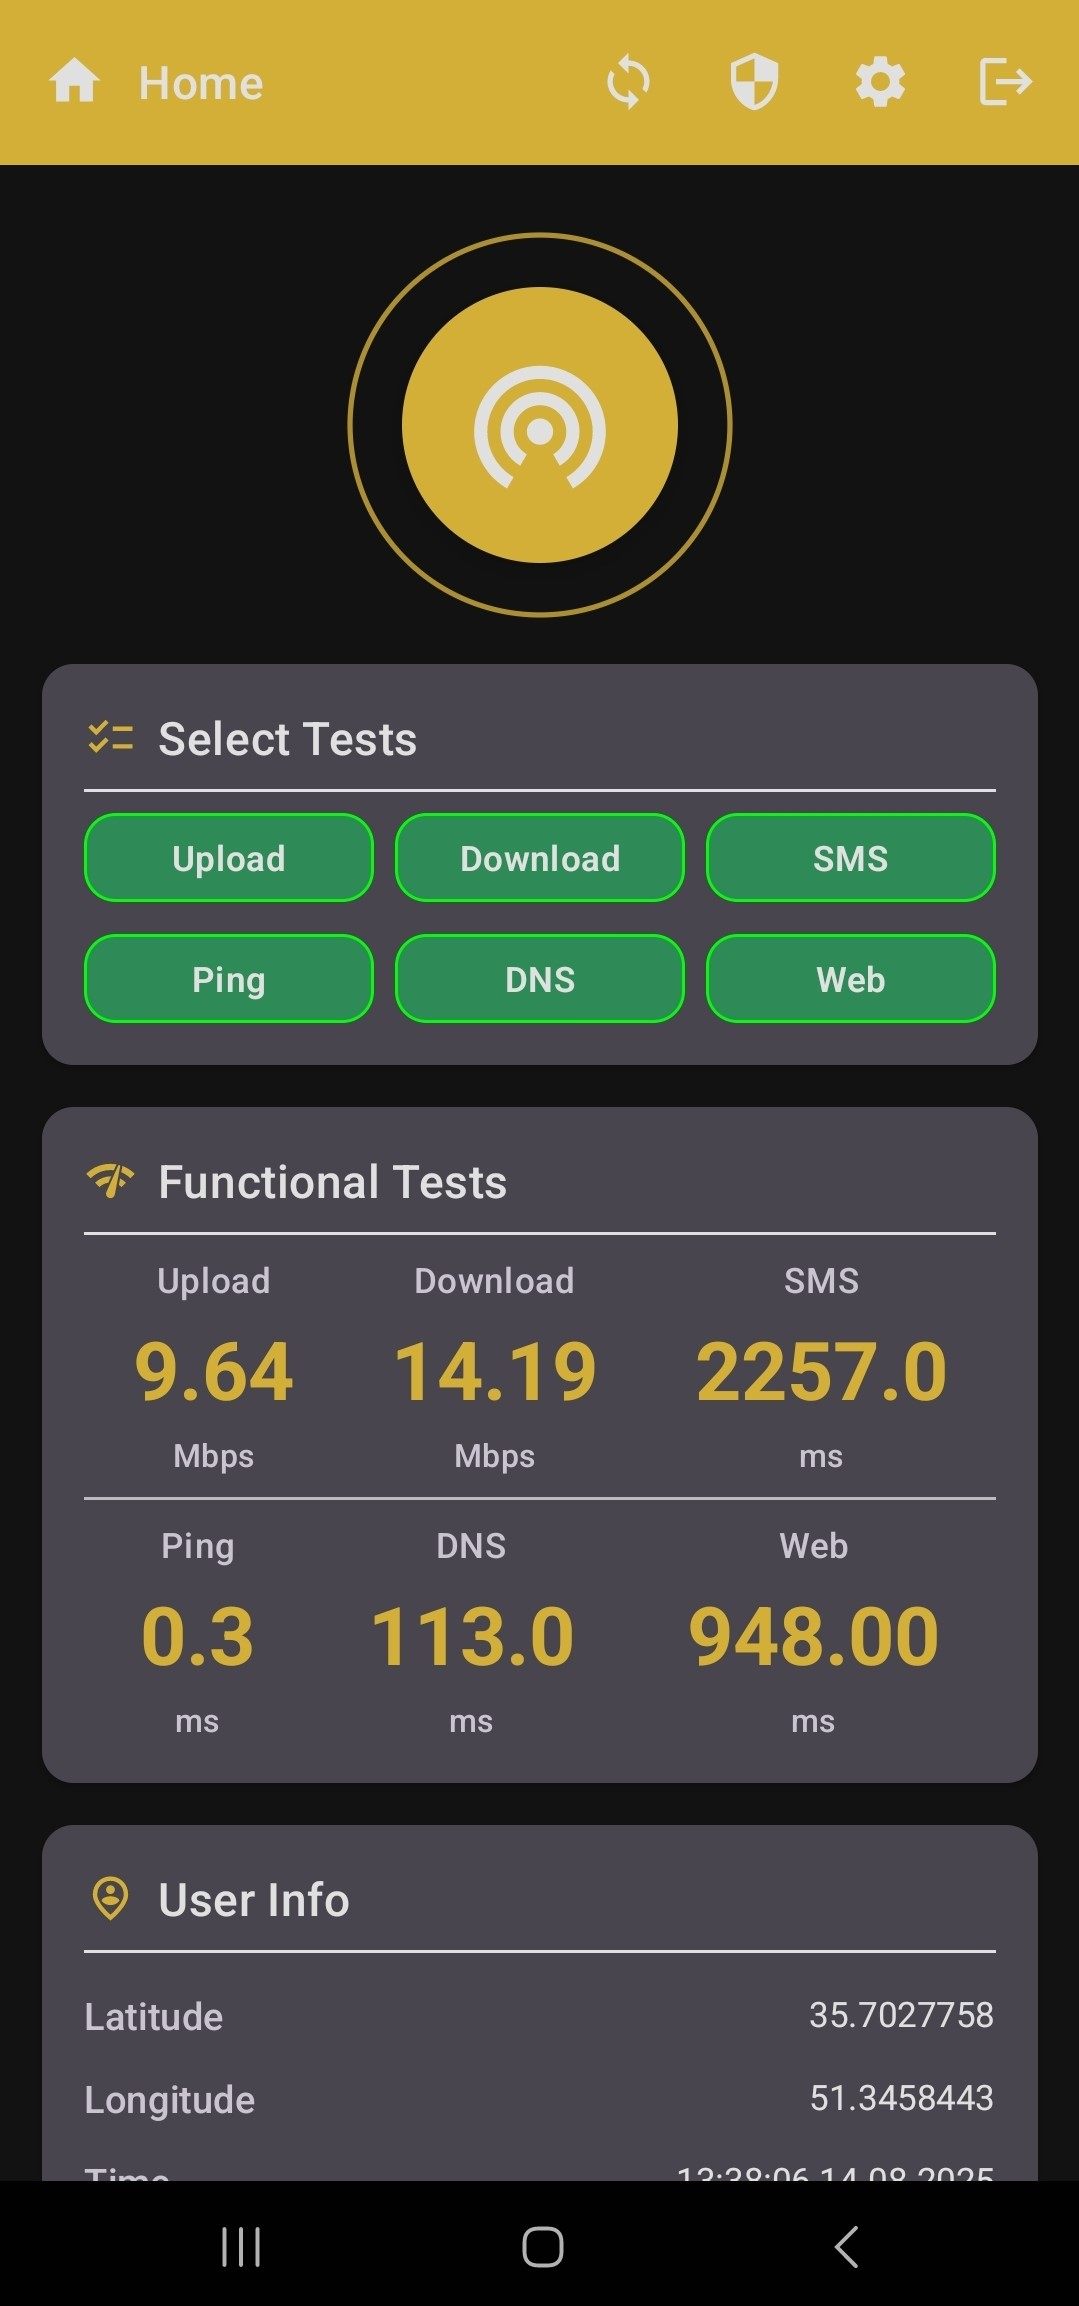
\includegraphics[width=0.4\textwidth]{images/home-filled.jpg}
			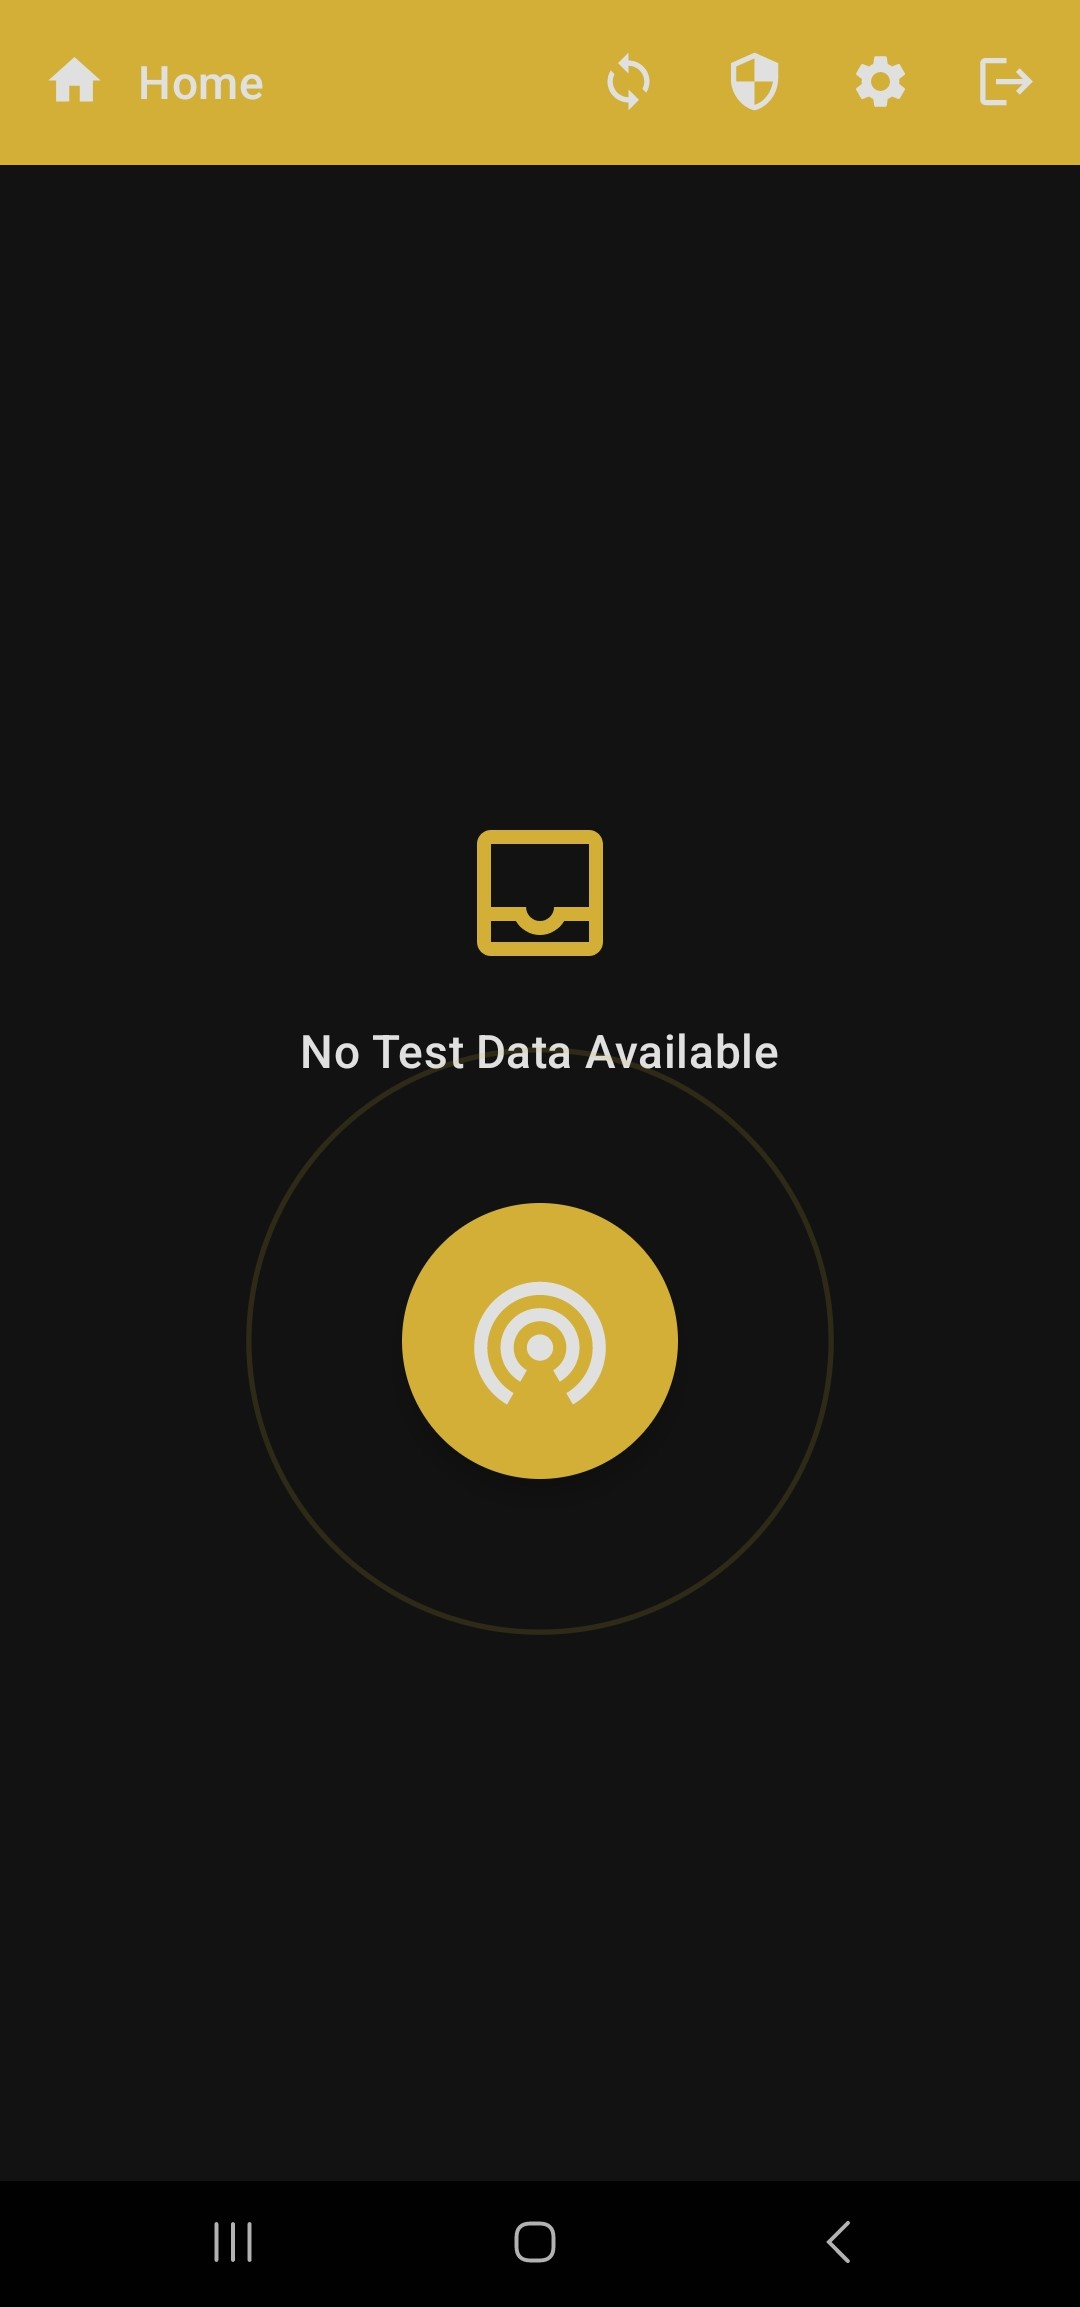
\includegraphics[width=0.4\textwidth]{images/home-empty.jpg}
		\end{center}
		
	\item  بازنشانی رمز عبور: برای بازنشانی رمز عبور در این برنامه نیاز است که ابتدا در صفحه Login که صفحه ابتدایی برنامه پس از دادن دسترسی‌های گفته شده است لینک \lr{Forgot Password?} را انتخاب کرده تا به صفحه زیر منتقل شوید:
		\begin{center}
			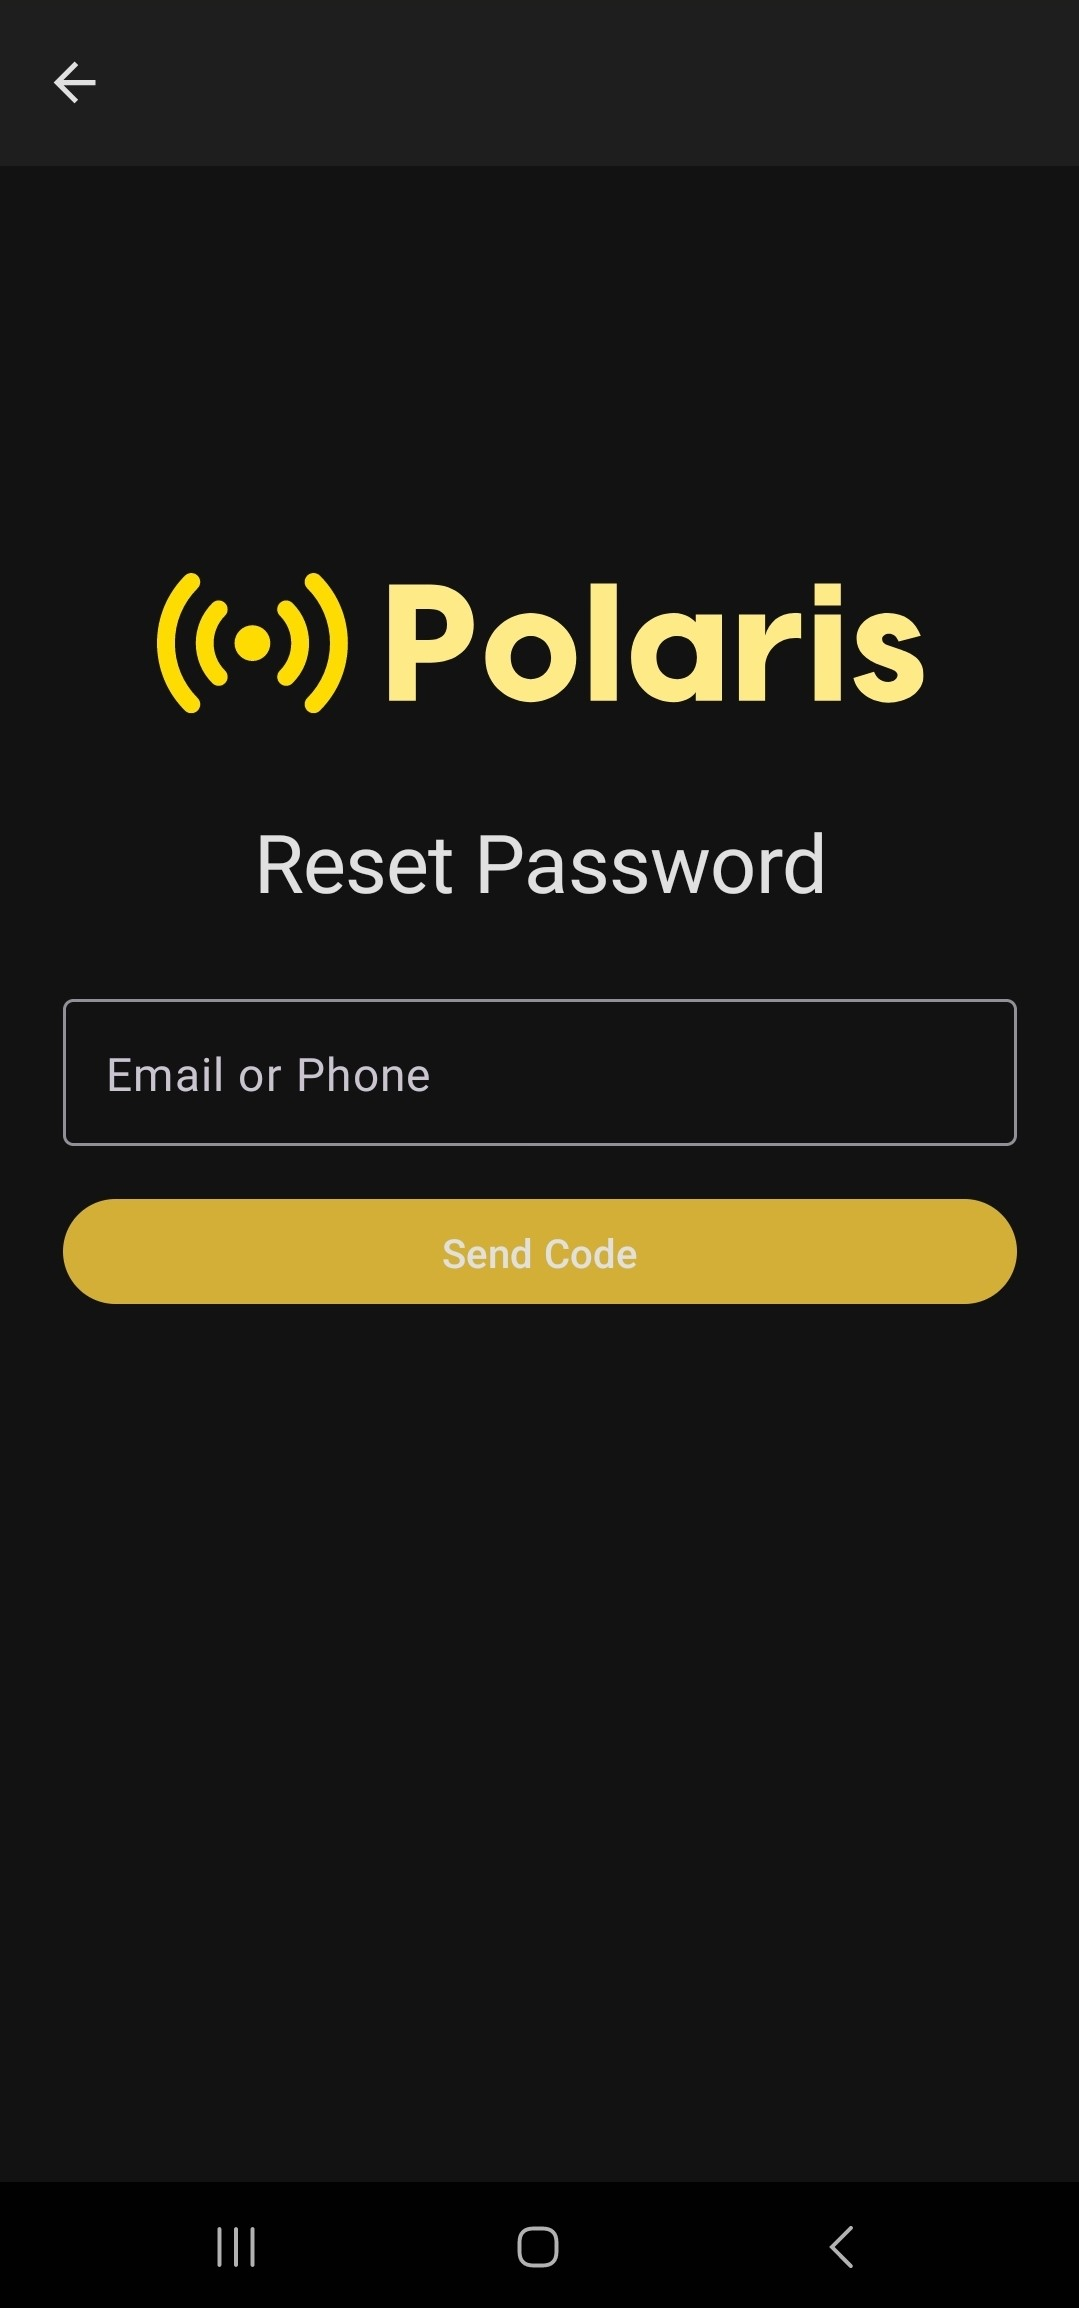
\includegraphics[width=0.4\textwidth]{images/reset-pass-empty.jpg}
		\end{center}
	لازم به ذکر است که از طریق دکمه فلش به سمت چپ می‌توان در هر مرحله به صفحه پیشین یا مرحله قبلی در بازنشانی رمز عبور برگشت.
	\begin{itemize}
		\item  مرحله ۱ (احراز هویت):
		در این مرحله ابتدا نیاز است که پست الکترونیک یا شماره موبایل وارد شود تا کدی برای احراز هویت کاربر به ایمیل او ارسال شود. پس از وارد کردن این مشخصه روی دکمه \lr{Send Code} کلیک کنید تا به مرحله بعدی بروید.
		\item  مرحله ۲ (تأیید):
		پس از وارد کردن مشخصه در مرحله پیشین و موفقیت آمیز بودن درخواست کاربر پیام موفقیت آمیز بودن نمایش داده شده و صفحه زیر ظاهر می‌شود:
			\begin{center}
				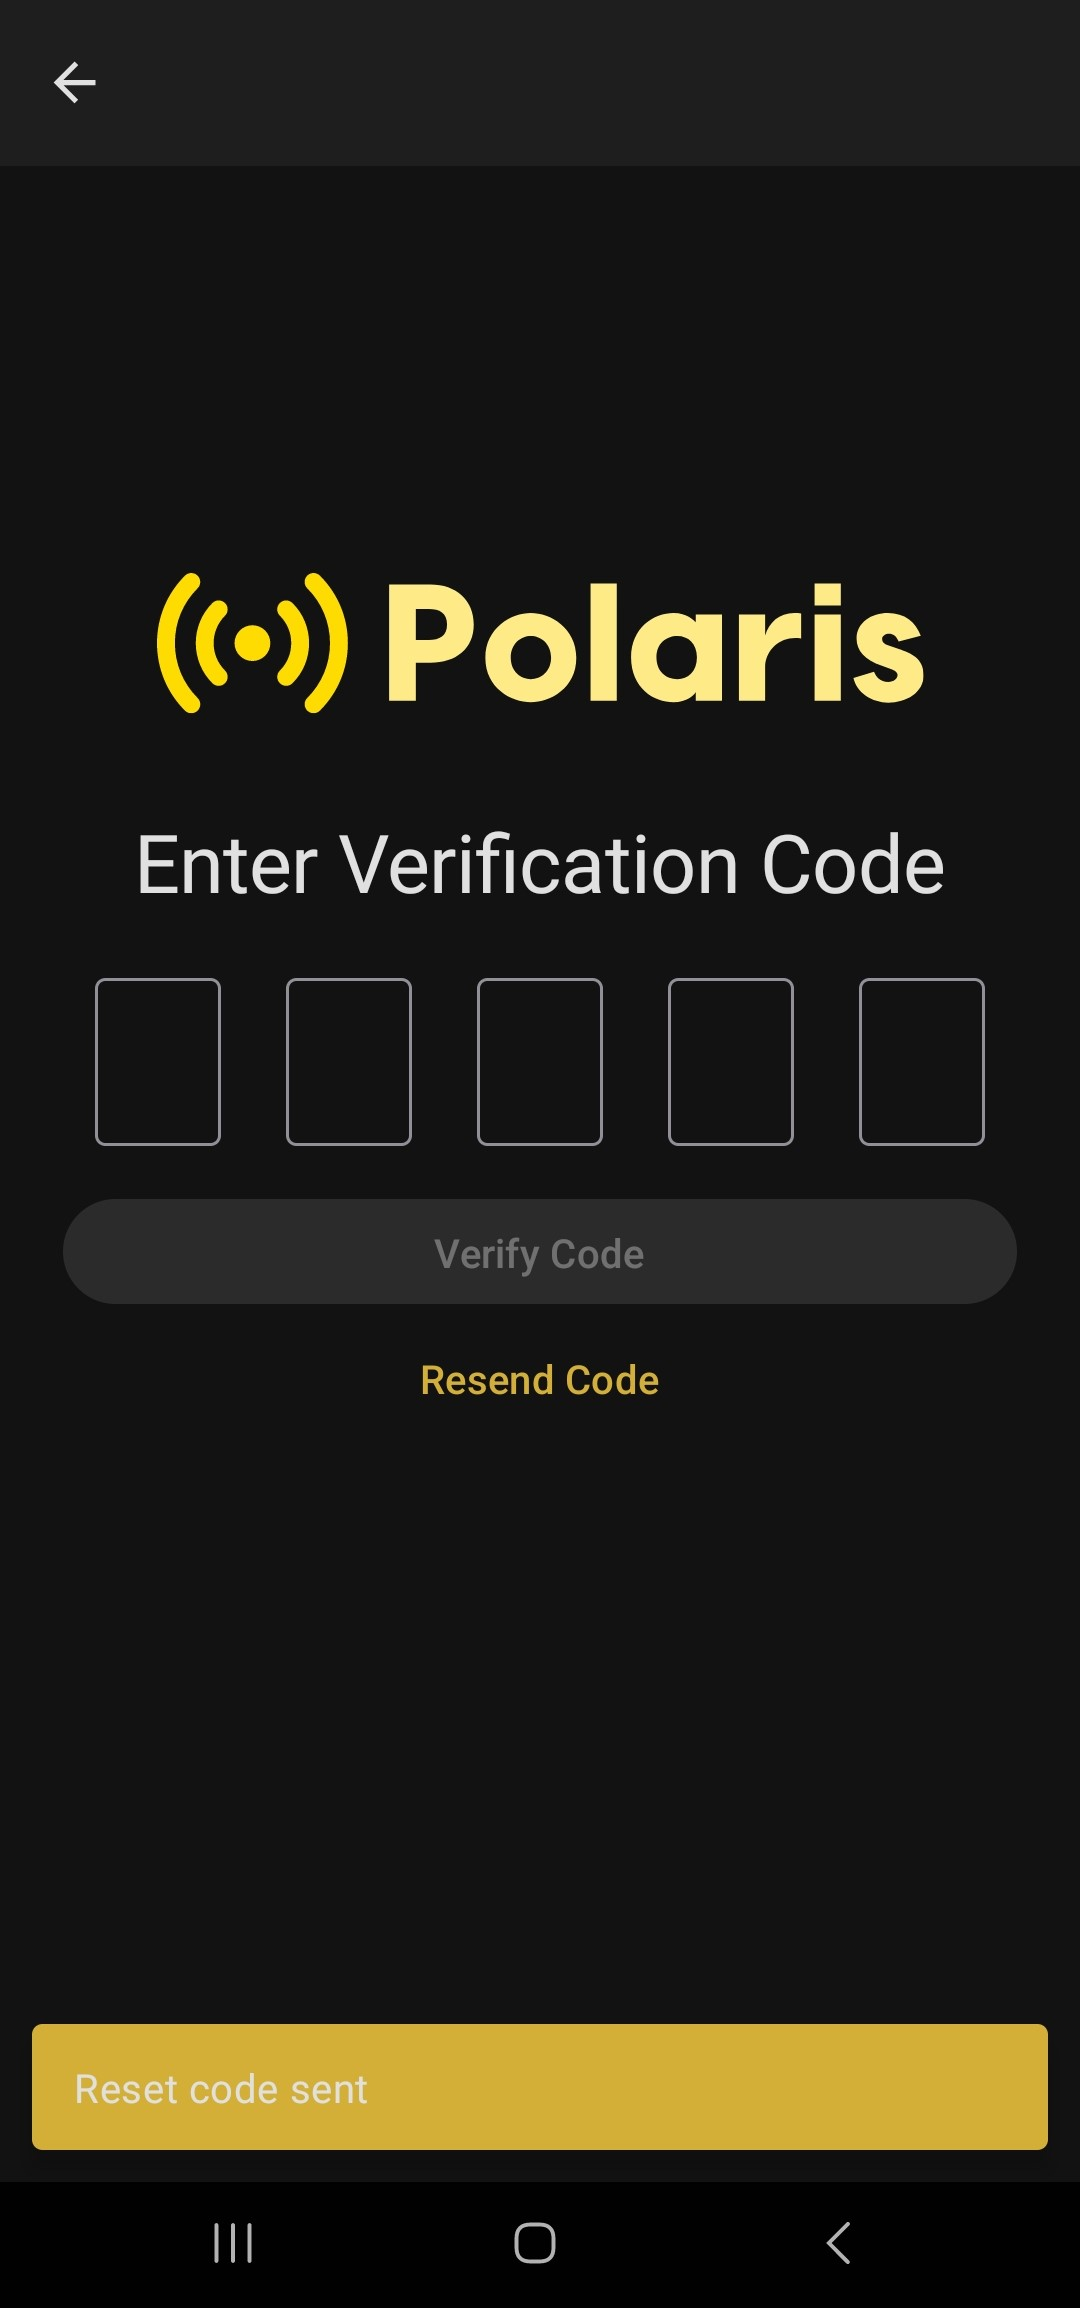
\includegraphics[width=0.4\textwidth]{images/verification-empty.jpg}
			\end{center}
		در این مرحله نیاز است کد ارسال شده به پست الکترونیک کاربر وارد شود و سپس بر روی دکمه \lr{Verify Code} کلیک شود. در صورت عدم دریافت کد می‌توان بر روی لینک \lr{Resend Code} کلیک کرد تا کد احراز هویت مجدد ارسال شود و یا با کلیک بر روی فلش در بالای برنامه به مرحله پیشین رفت و مشخصه پست الکترونیک یا شماره همراه را اصلاح نمود.
		\item  مرحله ۳ (تغییر رمز عبور): پس از وارد کردن کد 5 رقمی ارسالی به پست الکترونیکی کاربر و در صورت موفقیت آمیز بودن آن پیام مناسبی نمایش داده می‌شود و صفحه به شکل زیر در می‌آید:
			\begin{center}
				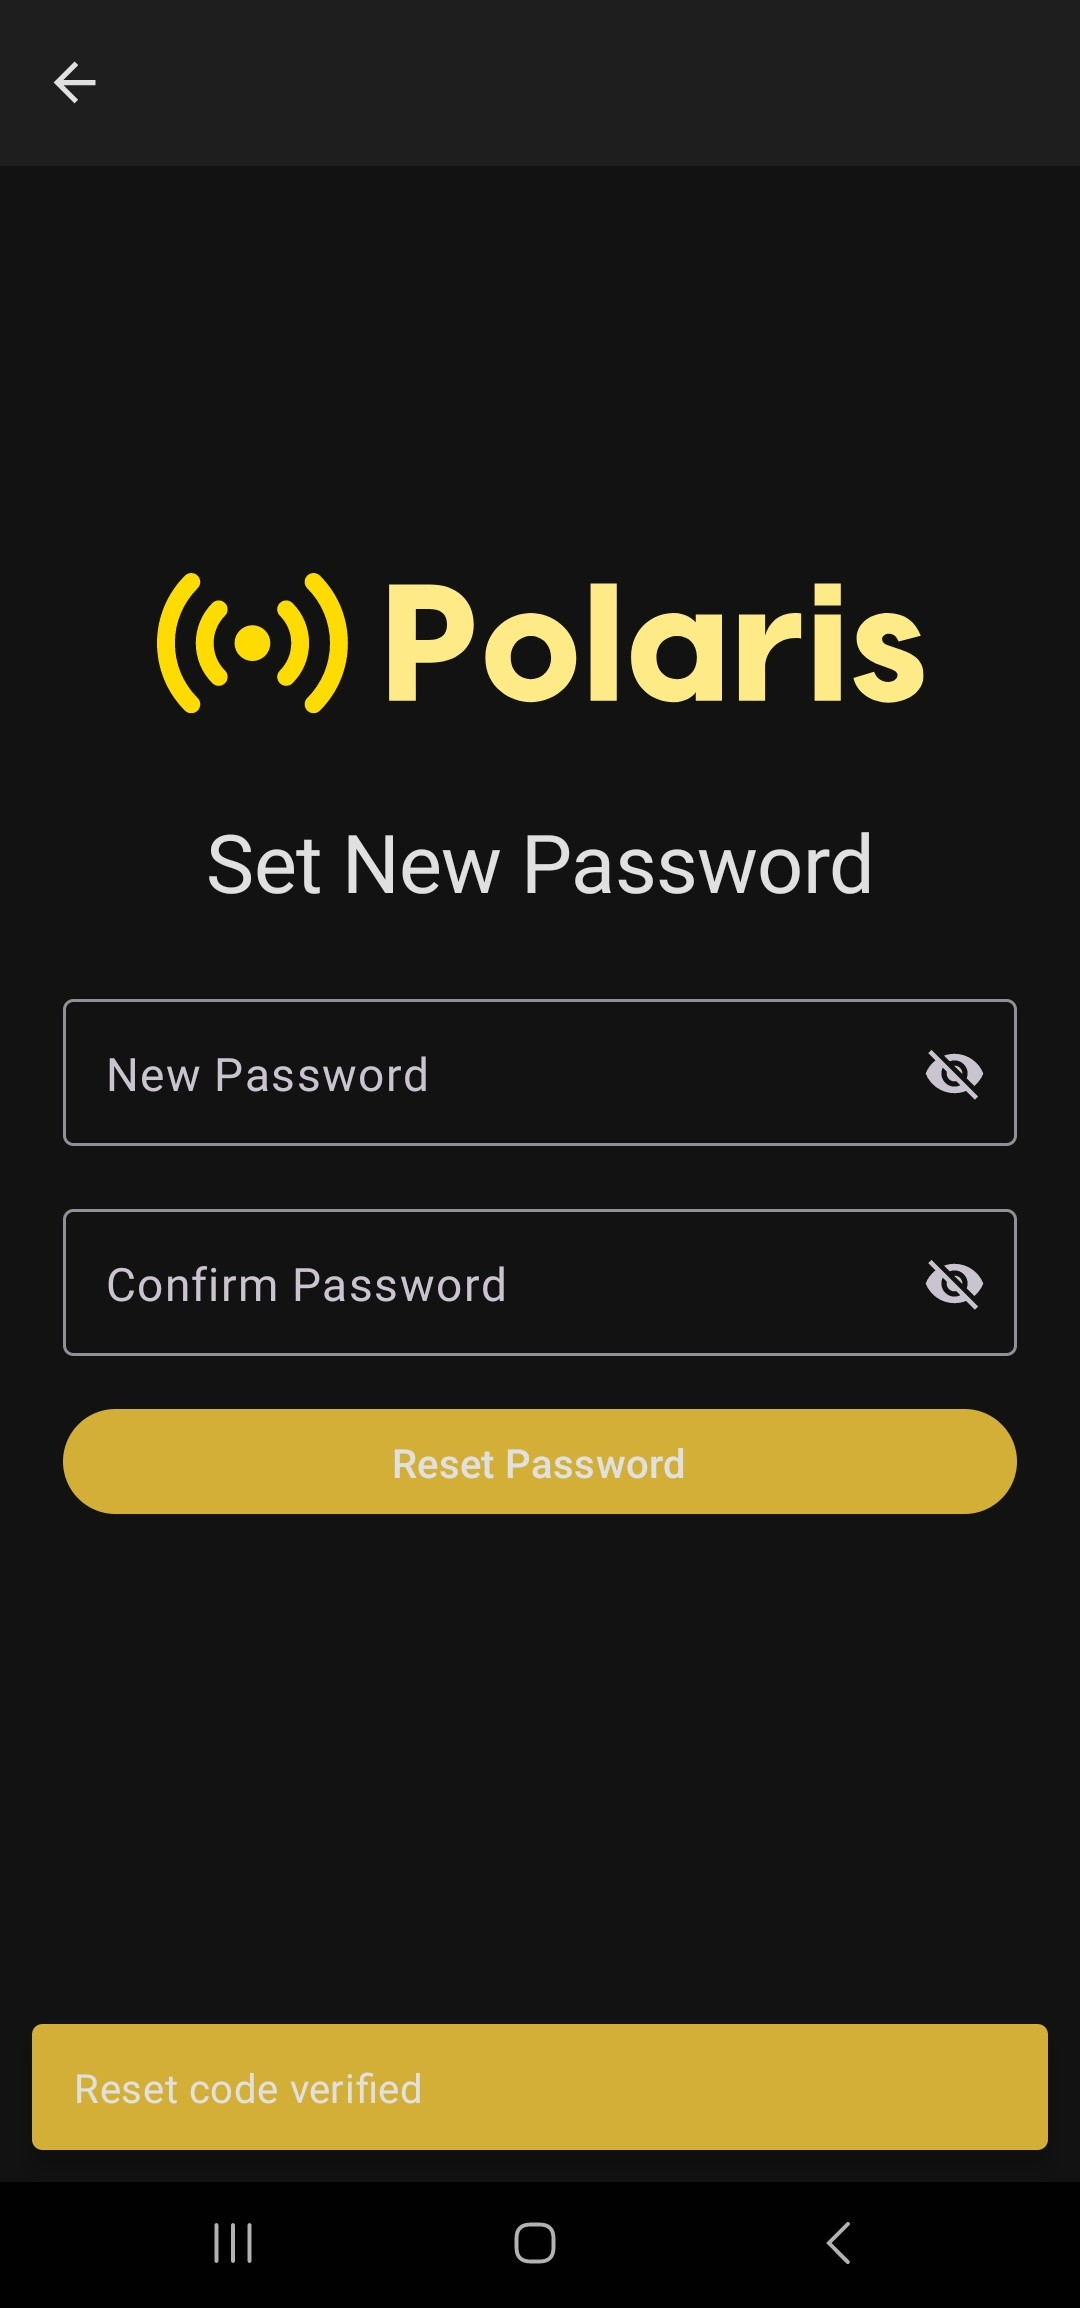
\includegraphics[width=0.4\textwidth]{images/new-pass-empty.jpg}
			\end{center}
		در این مرحله می‌بایست رمز جدید مناسب(به طول حداقل 8 کاراکتر) و تکرار آن وارد شود و بر روی دکمه \lr{Reset Password} کلیک شود. در صورت با خطا مواجه شدن این درخواست پیام خطا نمایش داده شده و در صورت موفقیت آمیز بودن پیام مناسب ظاهر می‌شود:
			\begin{center}
				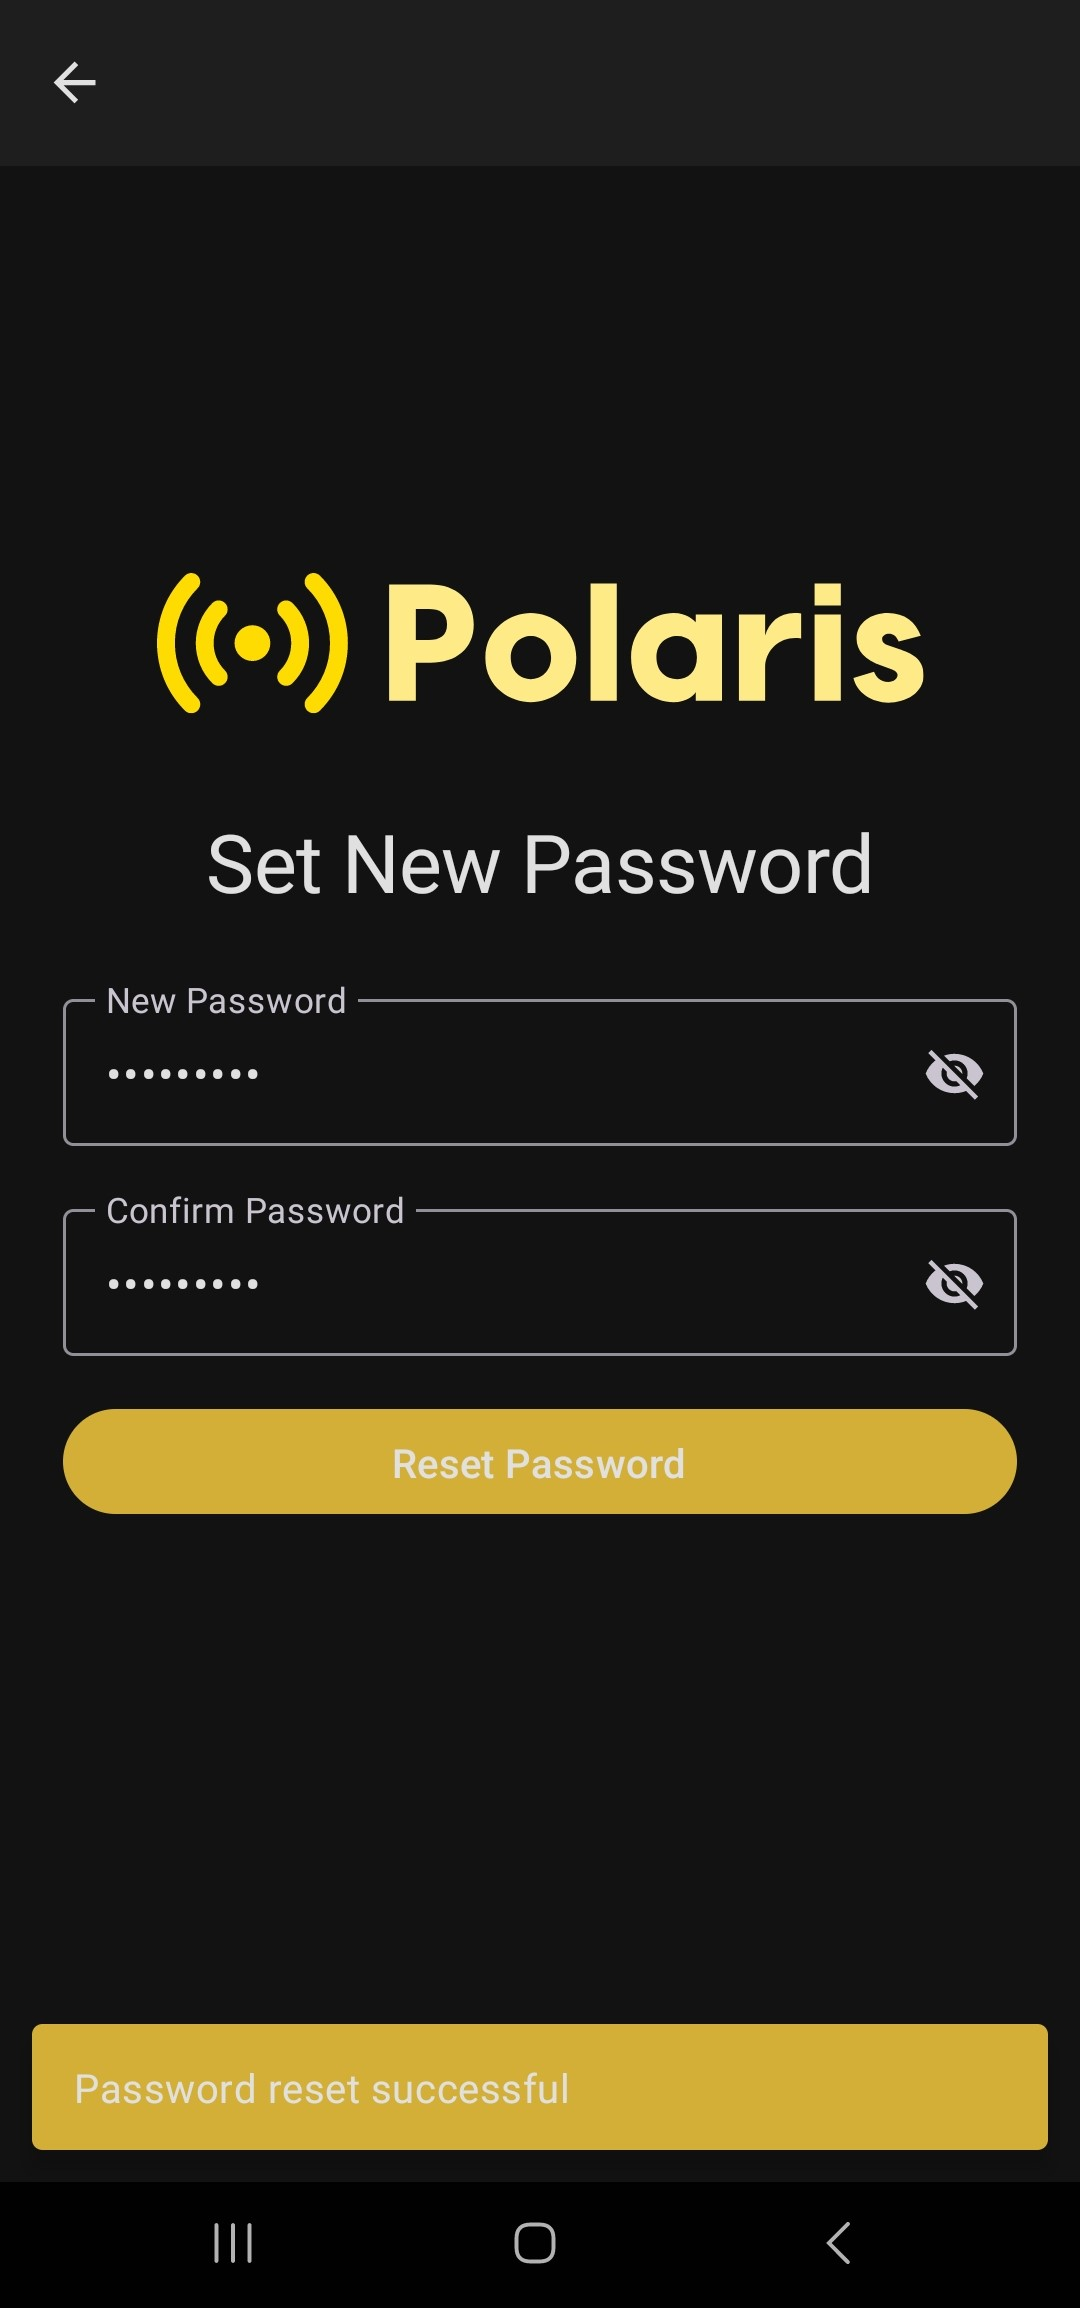
\includegraphics[width=0.4\textwidth]{images/new-pass-success.jpg}
			\end{center}
		سپس بعد از کمی تاخیر به صفحه Login هدایت می‌شوید که نیاز است مجدد با رمز جدید وارد حساب کاربری خود شوید.
	\end{itemize}
\end{itemize}
\section{استفاده از برنامه}
\begin{itemize}
	\item  مرور کلی صفحه اصلی: توضیح طرح‌بندی و ویژگی‌های اصلی صفحه اصلی.
	\item  اقدامات در صفحه اصلی:
	\begin{itemize}
            \item  اندازه گیری پارامترها و انجام تست‌ها:
                در صفحه اصلی، امکان اندازه گیری پارامتر‌های شبکه، انجام تست‌های دلخواه و همچنین مشاهده نتایج آخرین ارزیابی صورت گرفته وجود دارد.
                در این صفحه با کلیک بر روی دکمه حاضر در صفحه تمام پارامتر‌های شبکه اندازه گیری می‌شوند و در صورت انتخاب کاربر، تست‌های دلخواه او که در پنل \lr{Select Tests} انتخاب شده اند نیز اجرا می‌شوند. تست‌های انتخاب شده به رنگ سبز نمایش داده می‌شوند. شایان ذکر است در اجرای \lr{background} نیز تست‌های انتخاب شده در این پنل اجرا می‌شوند. 
                تصویر زیر نمونه‌ای از اجرای تست های \lr{Upload Throughput}، \lr{Download Throughput} و \lr{SMS Delivery} را نشان می‌دهد.
            \begin{center}
			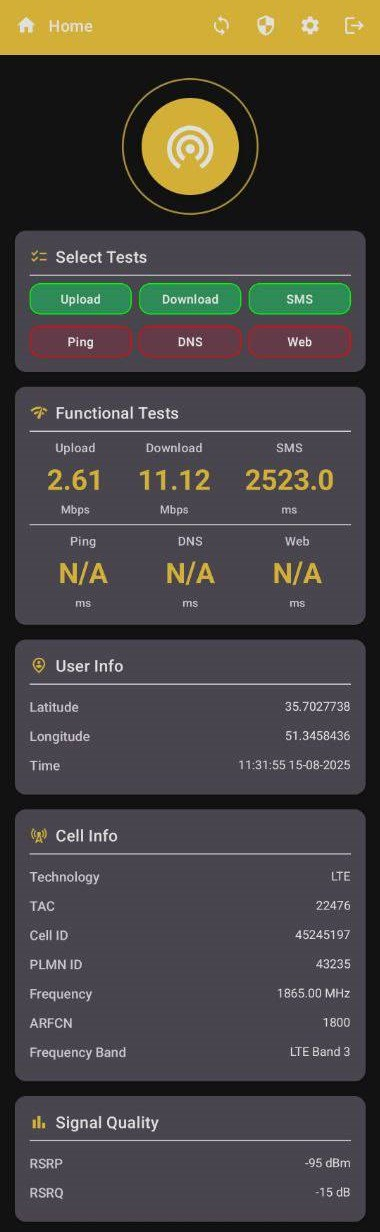
\includegraphics[width=0.4\textwidth]{images/TestResults.jpeg}
		\end{center} 
                نتایج تست‌های انجام شده در بخش \lr{Functional Tests} نشان داده شده است. با توجه به اینکه تنها ۳ تست مذکور انتخاب شده اند نتایج عددی فقط برای آنها ثبت شده است. در صورتی که تستی انتخاب نشده باشد و یا در اجرای تست انتخاب شده مشکلی به وجود بیاید نتیجه به صورت \lr{N/A} نمایش داده می‌شود.

                نتایج مربوط به پارامترهای شبکه در ۳ کارت جهت تفکیک بهتر و ارتقای کیفیت کاربری نمایش داده می‌شوند. کارت اول \lr{User Info} شامل موقعیت جغرافیایی دقیق و تاریخ ارزیابی است. کارت دوم \lr{Cell Info} اطلاعات مربوط به سلول و اتصال به آن است. به طور دقیق تر شامل نسل مربوطه، کد موقعیتی آن، شناسه سلول، شناسه مربوط به کشور و اپراتور، فرکانس و باند فرکانسی می‌باشد. کارت سوم \lr{Signal Quality} کیفیت اتصال را نشان میدهد که با توجه به نسل مورد نظر پارامتر مرتبط به آن نمایش داده می‌شود.
        
		\item  تازه‌سازی داده‌ها:
		در صفحه خانه میتوان اولین دکمه بالا از سمت چپ که به شکل دو فلش است را کلیک کرد و داده‌ها را با آخرین اندازه‌گیری انجام شده روی تلفن همراه همگام نمود:
		\begin{center}
			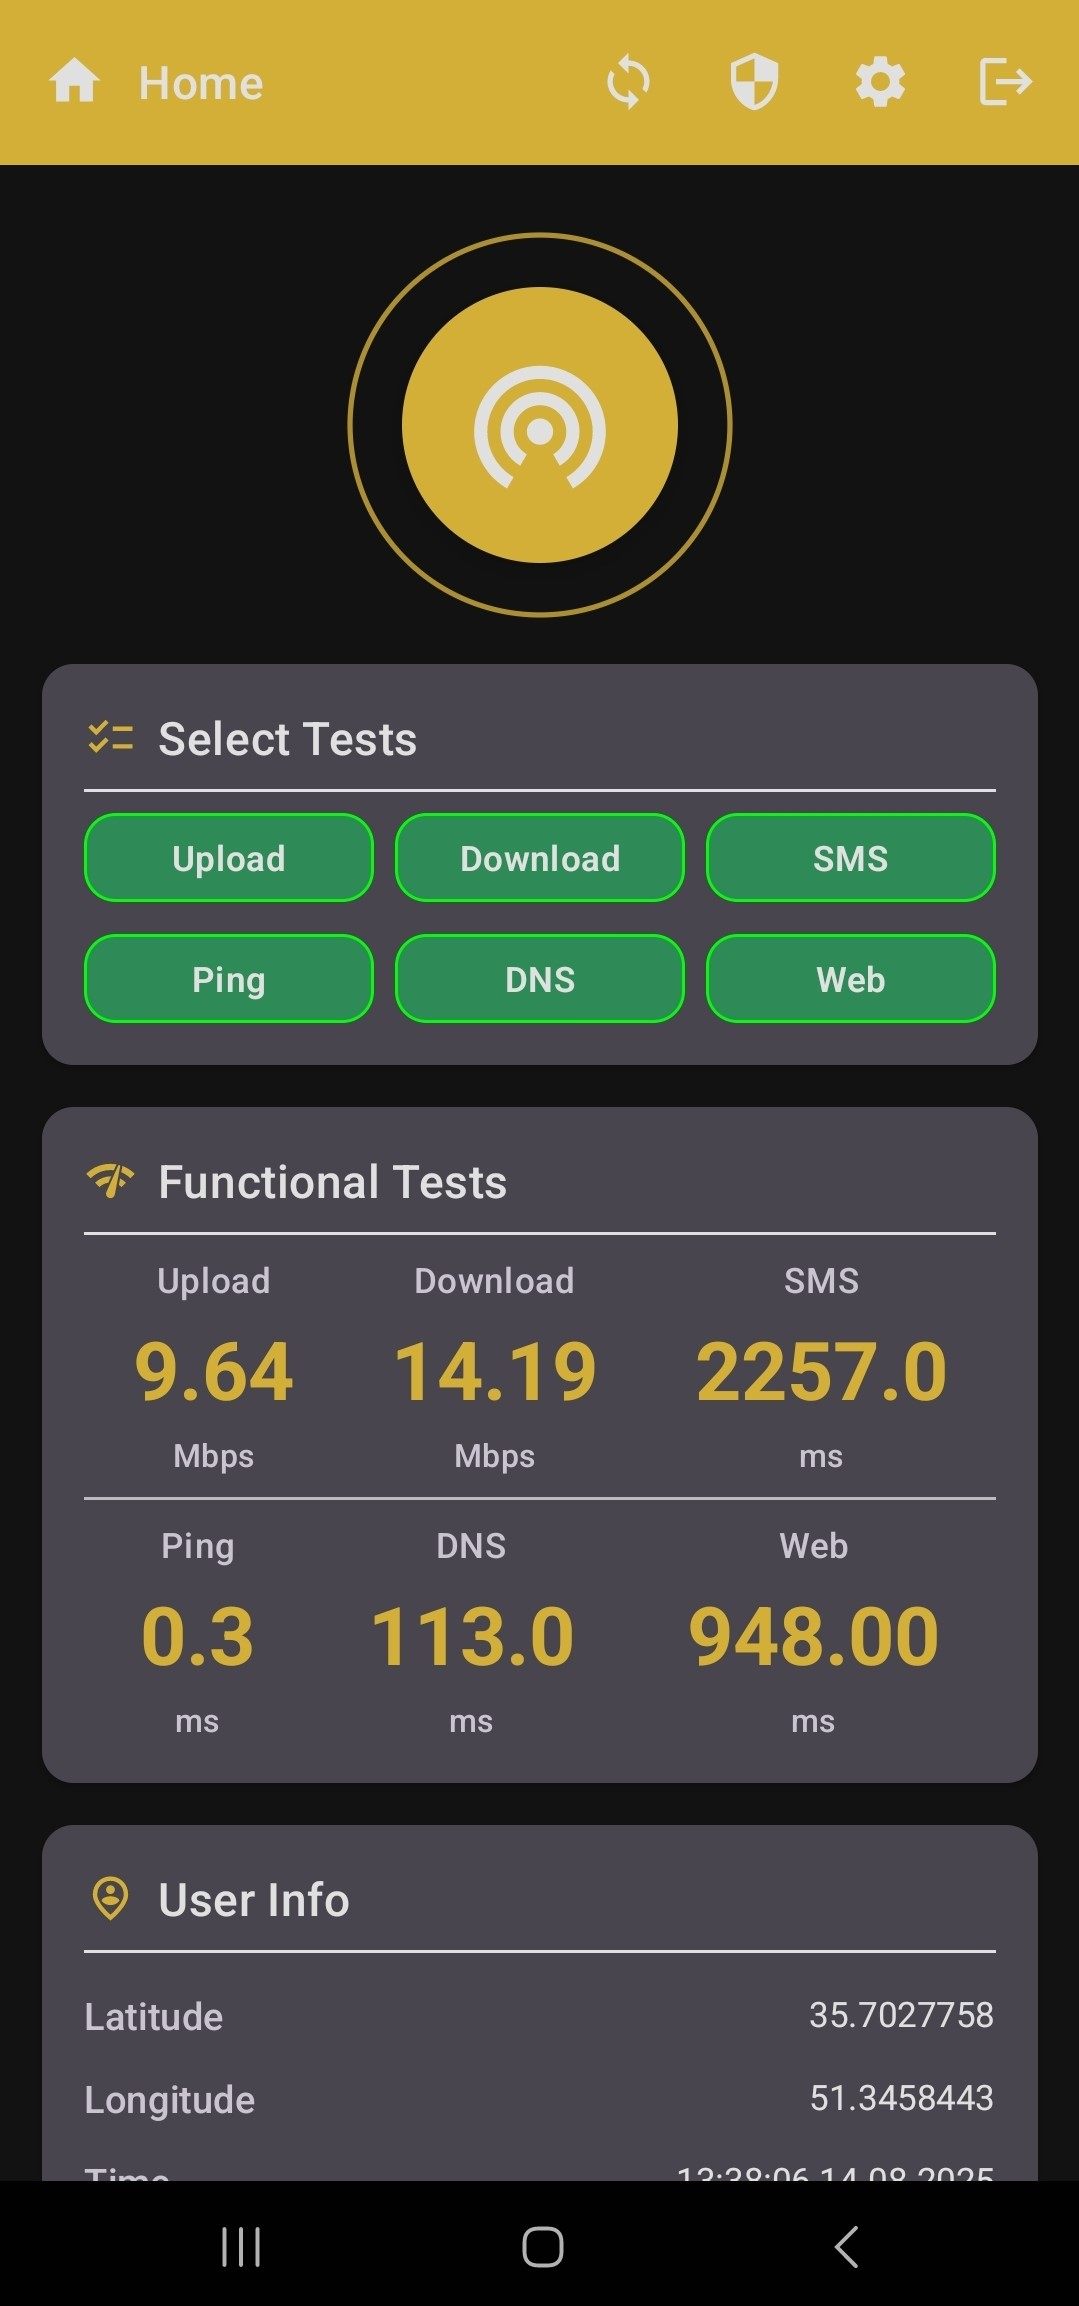
\includegraphics[width=0.4\textwidth]{images/home-filled.jpg}
		\end{center}

            \item  بررسی مجوزها:
		در صفحه خانه میتوان دومین دکمه بالا از سمت چپ که به شکل سپر است را کلیک کرد و صفحه بررسی مجوزهای مورد نیاز برنامه را مشاهده کرد و در صورت ناقص بودن دسترسی‌ها، آن‌ها را کامل کرد.
        همانطور که در تصویر زیر مشاهده میکنید، در بالای صفحه کارت خلاصه ای از وضعیت دسترسی‌ها وجود دارد و پایین تر از آن لیستی از این دسترسی‌ها، دلیل نیاز به آنها و وضعیتشان که مستقیما و الزاما توسط خود کاربر باید داده شوند وجود دارد. شایان ذکر است برخی دسترسی‌‌های تعریف شده در برنامه مستقیما اخذ میشوند و نیازی به اجازه کاربر ندارند که در اینجا نمایش داده نشده‌اند.
            \begin{center}
		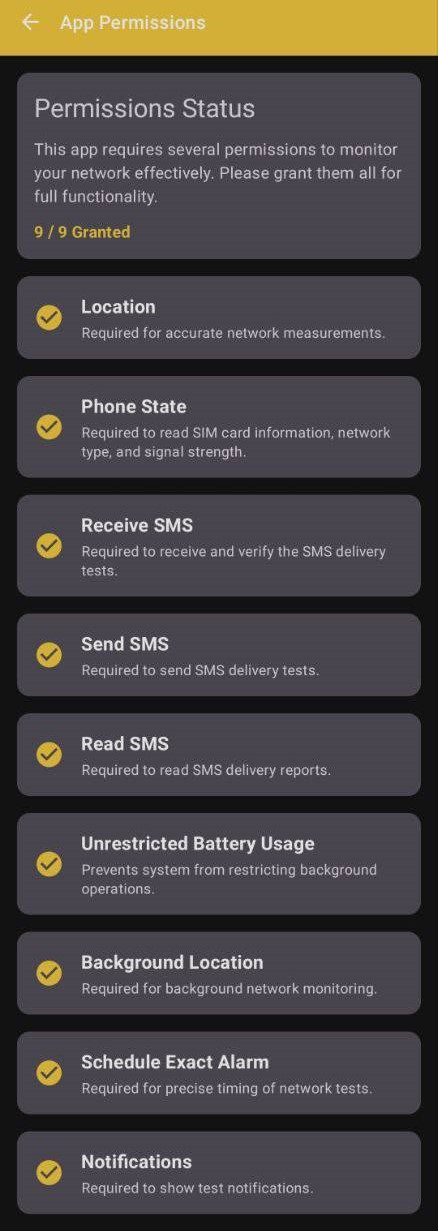
\includegraphics[width=0.4\textwidth]{images/PermissionAll.jpeg}
		\end{center}
        
        تصویری که در ادامه مشاهده می‌کنید مربوط به زمانی است که کاربر دسترسی اعلان‌ها (\lr{Notification}) را نداده است. (برای نسخه‌های ۱۳ به بعد اندروید) همانطور که در تصویر مشخص است این عدم دسترسی به کاربر اطلاع داده شده است. (این فرآیند برای همه مجوزهاست.)
            \begin{center}
		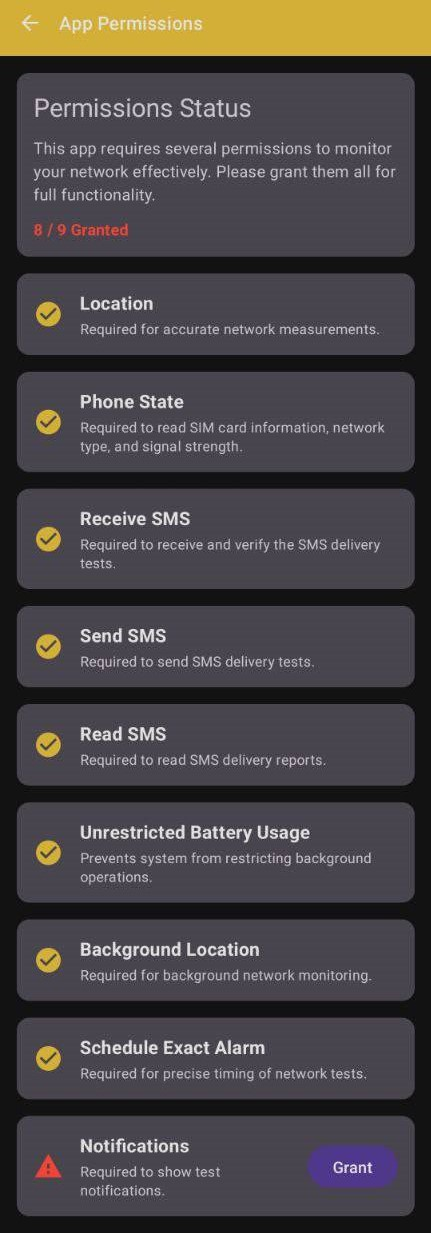
\includegraphics[width=0.4\textwidth]{images/Permission.jpeg}
	    \end{center}
        در این قسمت و در کارت خود دسترسی \lr{Notification} با کلیک بر روی دکمه \lr{Grant} صفحه ای باز میشود که کاربر را جهت اخذ دسترسی راهنمایی میکند. شایان ذکر است که علی رغم اطلاع و راهنمایی در این صفحه، هنگام مراجعه بعدی کاربر به برنامه در صورتی که دسترسی ای داده نشده باشد از او درخواست می‌شود. (این فرآیند برای همه مجوزهاست.)
            \begin{center}
		  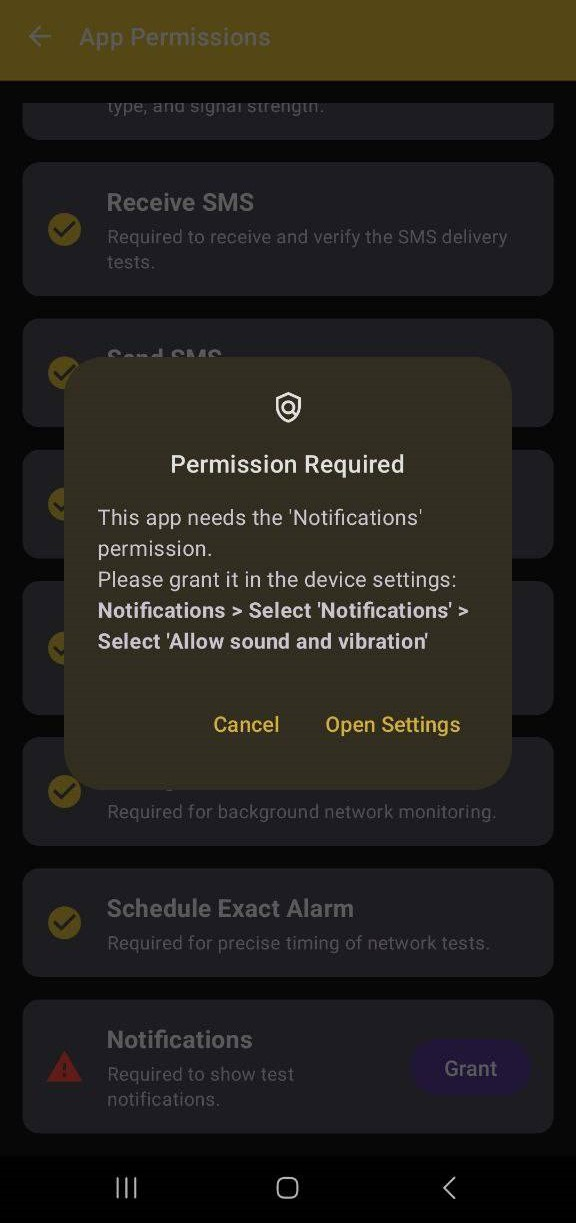
\includegraphics[width=0.4\textwidth]{images/Grant.jpeg}
	    \end{center}
		
		\item  تنظیمات:
		در صفحه خانه میتوان دکمه تنظمیات در بالا صفحه را کلیک کرد و جهت تغییر پیشفرض‌ها اقدام کرد. در صورتی که دستگاه کاربر از بیش از ۱ سیمکارت پشتیبانی بکند و به تبع آن چندین سیمکارت در دستگاه کاربر موجود باشد، کاربر میتواند در این صفحه سیمکارت مورد نظر جهت ارزیابی را انتخاب کند. به طور پیشفرض سیمکارت اول انتخاب شده است.
        با توجه به امکان سینک کردن داده‌ها با خدمتگزار در بکگراند، کاربر می‌تواند بازه‌های زمانی مطلوب جهت این کار را از میان گزینه‌های موجود (۱۵ دقیقه، ۳۰ دقیقه، ۱ ساعت، ۶ ساعت، ۱۲ ساعت و ۲۴ ساعت) انتخاب کند. بازه زمانی مورد استفاده به صورت پیشفرض ۳۰ دقیقه است.
         بخش پایانی تنظیمات مربوط به تست‌هاست. تست‌های مربوط به گذردهی فراسو و فروسو با تبادل داده میان دستگاه کاربر و خدمتگزار \lr{Polaris} انجام میشود و لذا مسیر و حجم تبادل داده ثابت است. در مورد تست پیامک باید گفت این تست بر روی سیمکارت انتخاب شده در بخش اول انجام میشود و شماره مقصد جهت ارسال پیامک به آن و ارزیابی زمان تحویل توسط کاربر در این بخش انجام می‌شود. شماره وارد شده باید به متعلق به ایران و معتبر باشد در غیر اینصورت تست پیامک با شماره پیشفرض \lr{Polaris} انجام می‌شود. سایر تست‌های تعریف شده در برنامه نیاز به یک مقصد مشخص دارند. (آدرس \lr{Ping}، \lr{DNS} و \lr{Web Response}) برای این تست ها نیز لازم است کاربر آدرسی معتبر وارد کند و در غیر اینصورت از آدرس‌های پیشفرض \lr{Polaris} استفاده می‌شود. در زیر تصویر صفحه تنظیمات و مقادیر پیشفرض آن را مشاهده می‌کنید:
         
            \begin{center}
			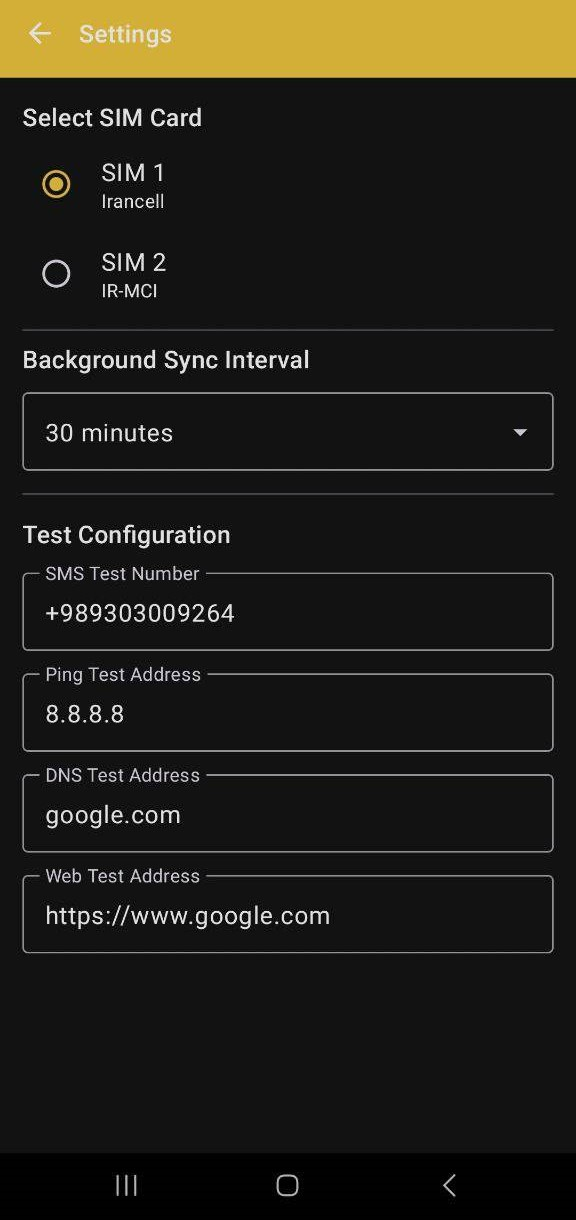
\includegraphics[width=0.4\textwidth]{images/Settings.jpeg}
		\end{center}
        
		\item  خروج از حساب:
		در صفحه خانه میتوان اولین دکمه بالا از سمت راست که به شکل خروج است را کلیک کرد و از حساب خود خروج انجام داد:
			\begin{center}
				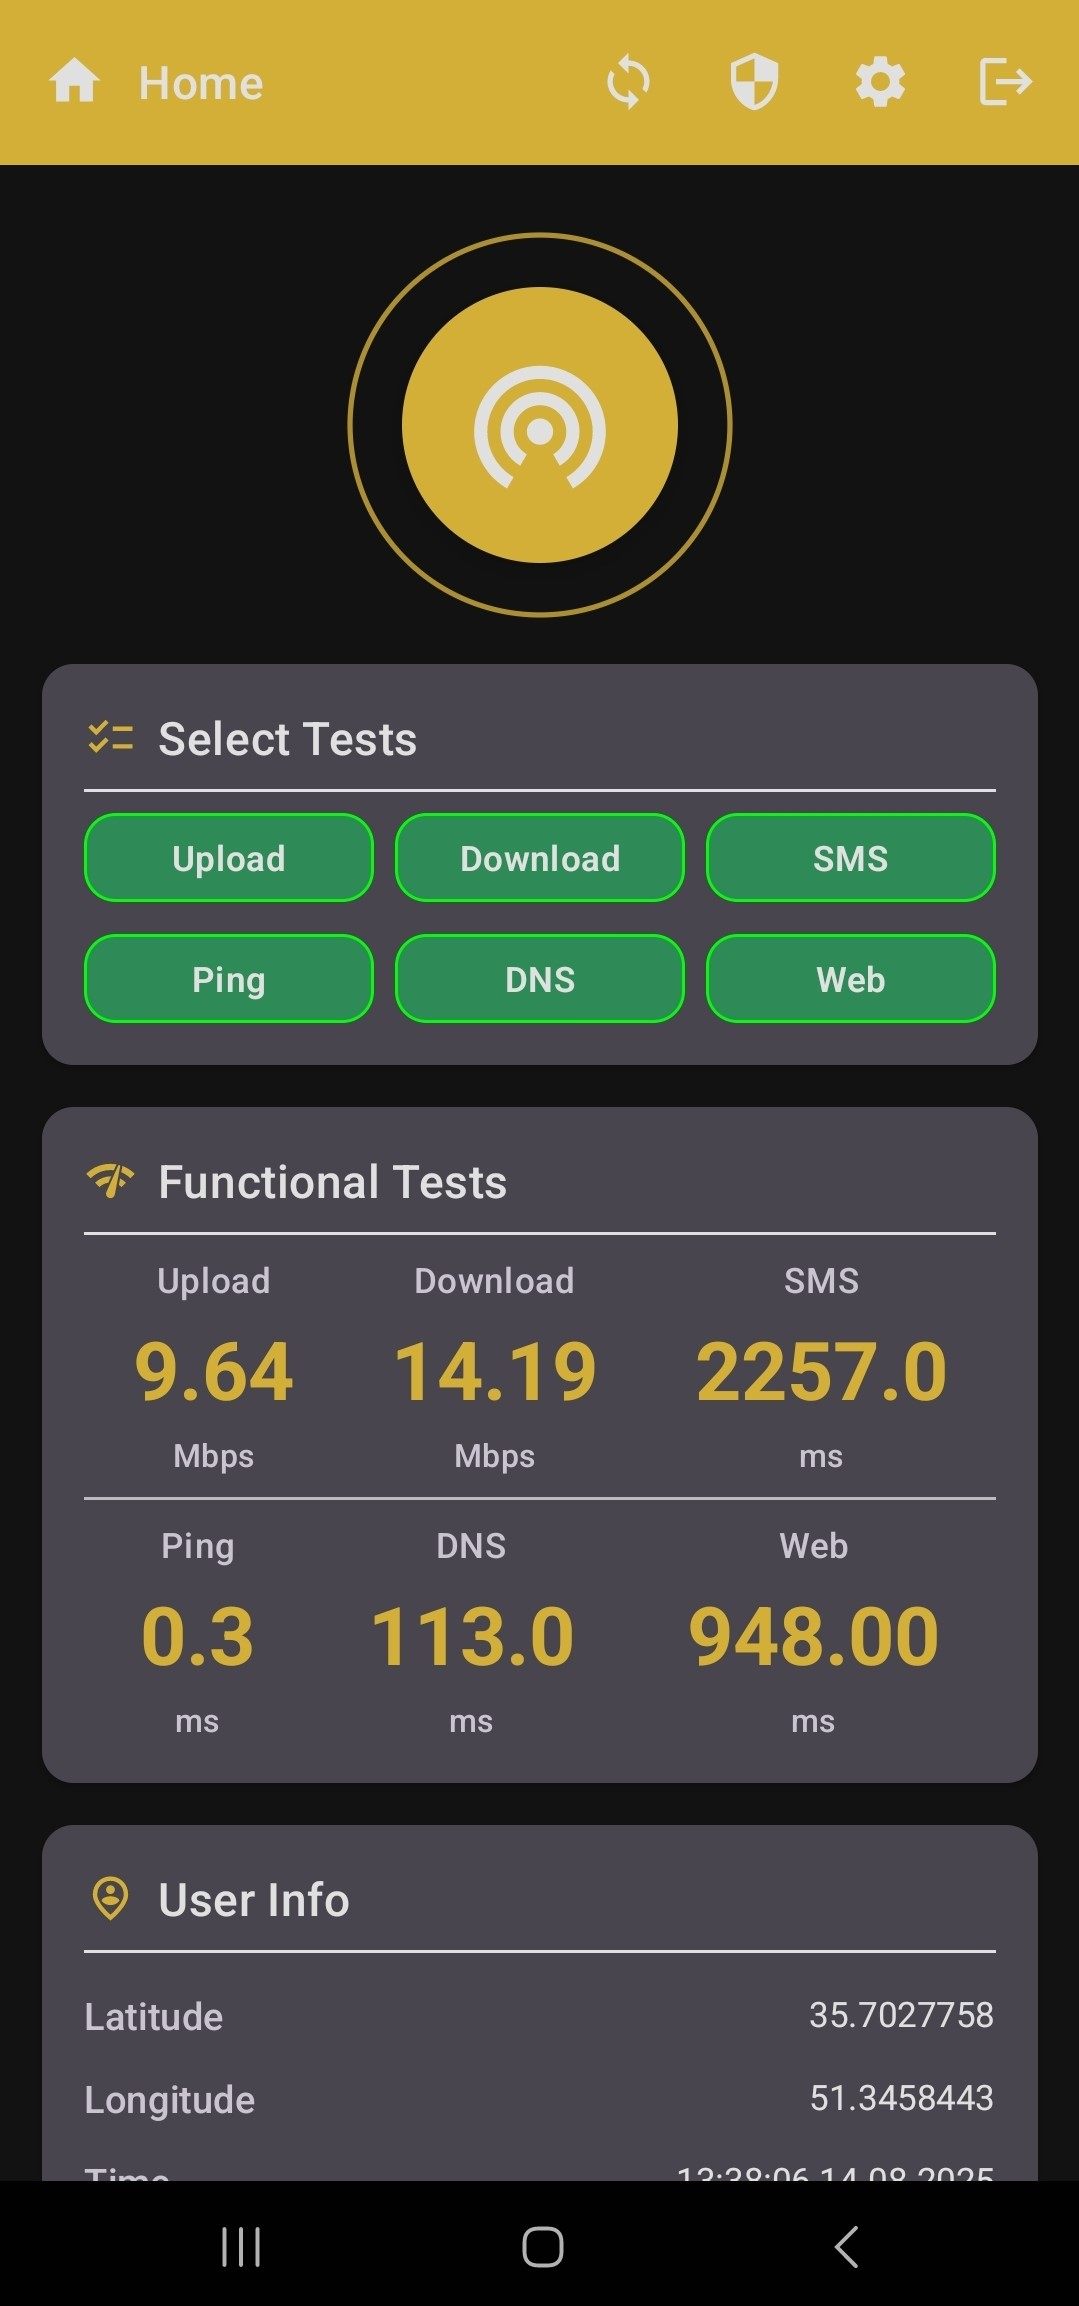
\includegraphics[width=0.4\textwidth]{images/home-filled.jpg}
			\end{center}
		که پس از آن مجدد وارد صفحه Login می‌شویم.
	\end{itemize}
\end{itemize}